    \documentclass[
        fleqn,
        usenatbib,
    ]{mnras}
    \usepackage{
        amsmath,
        amssymb,
        newtxtext,
        newtxmath,
        ae, aecompl,
        graphicx,
        booktabs,
    }
    \usepackage[T1]{fontenc}
    \usepackage[
        labelfont=bf, % caption names are labeled in bold
        font=scriptsize % smaller font for captions
    ]{caption}

    \newcommand*{\rd}[2]{\frac{\mathrm{d}#1}{\mathrm{d}#2}}
    \newcommand*{\pd}[2]{\frac{\partial#1}{\partial#2}}
    \newcommand*{\md}[2]{\frac{\mathrm{D}#1}{\mathrm{D}#2}}
    \newcommand*{\at}[1]{\left.#1\right|}
    \newcommand*{\abs}[1]{\left|#1\right|}
    \newcommand*{\ev}[1]{\langle#1\rangle}
    \newcommand*{\p}[1]{\left(#1\right)}
    \newcommand*{\s}[1]{\left[#1\right]}
    \newcommand*{\z}[1]{\left\{#1\right\}}
    \DeclareMathOperator*{\argmin}{argmin}
    \DeclareMathOperator*{\argmax}{argmax}
    \DeclareMathOperator*{\med}{med}

\title[Internal Gravity Wave Breaking in White Dwarf Binaries]{Internal Gravity Wave Breaking in White Dwarf Binaries}
\author[Y. Su et\ al.]{
Yubo Su,$^1$,
Daniel Lecoanet,$^2$
Dong Lai,$^1$
\\
$^1$ Cornell Center for Astrophysics and Planetary Science, Department of
Astronomy, Cornell University, Ithaca, NY 14853, USA
\\
$^2$ Princeton Center for Theoretical Science, Princeton University, Princeton,
NJ 08544, USA
}

\date{Accepted XXX\@. Received YYY\@; in original form ZZZ}

\pubyear{2019}

\begin{document}\label{firstpage}
\pagerange{\pageref{firstpage}--\pageref{lastpage}}
\renewcommand*{\sectionautorefname}{Section}
\maketitle


\begin{abstract}
    In sufficiently compact white dwarf binaries, dynamical tides raise a train
    of internal gravity waves that propagate towards the surface. We perform 2D
    numerical simulations of these waves undergoing nonlinear wave breaking in
    an incompressible, isothermal atmosphere. After an initial transient phase,
    we find that these waves induce a sharp transition between a non-rotating
    core and synchronously rotating envelope. We find evidence that the width of
    this transition layer is bound from below by the Kelvin-Helmholtz
    Instability. We provide analytical formulae for absorption and reflection of
    incident waves off the critical layer up to prefactors of order unity. These
    prefactors converge to constant values when artificial dissipation is
    decreased. We provide dimensionless criteria necessary to resolving momentum
    transfer within the critical layer. Finally, we speculate on the application
    of our model to tidal synchronization and heating in astrophysical systems.
\end{abstract}

\begin{keywords}
white dwarfs -- hydrodynamics -- binaries:close -- waves % chktex 8
\end{keywords}

\section{Introduction}

[Below copied from proposal, will rewrite]

Compact white dwarf (WD) binary systems, with orbital periods in the range of
minutes to hours, are important for a range of astrophysical problems. They are
the most important sources of gravitational waves (GWs) for the Laser
Interferometric Space Antenna (LISA) \citep{lisa}. They are also thought to
produce interesting optical transients such as underluminous
supernovae \citep{underlum}, Ca-rich fast transients \citep{carich}, and tidal
novae \citep{tidal_novae}. Most importantly, they have been proposed as the likely
progenitors of type Ia supernovae (e.g. \citep{Ia0,webbink} or more
recently \citep{Ia1,Ia2}). While presently only a few tens of compact WD binaries
are known \citep{lsst_wd}, \emph{Gaia} (currently gathering data) is expected to
expand the catalog to a few hundreds \citep{lsst_wd} (results based on
\emph{Gaia}'s second data release have already begun to
appear \citep{gaiaDD,gaiaDD2}), and the Large Synoptic Survey Telescope (LSST,
first light scheduled for 2020) will likely detect a few thousand
more \citep{lsst_wd}. These observations will significantly advance the
understanding of WD binaries and their evolution. My proposed theoretical and
computational research is well-timed to take advantage of these new advances.

In spite of the broad importance of WD binaries, the evolution of these systems
prior to their final mergers is not well understood. Much of this uncertainty
comes from our imprecise understanding of tidal interactions, which play an
important role during a compact WD binary's inspiral \citep{fullerII}. Previous
studies have shown that these interactions manifest as tidal excitation of
internal gravity waves (IGW), waves in the WD fluid restored by the buoyancy
force due to density stratification \citep{fullerI}. As these waves propagate
outwards towards the WD surface, they grow in amplitude until they break, as do
ocean waves on a shore, and transfer both energy and angular momentum from the
binary orbit to the outer envelope of the WD \citep{fullerI,fullerII}.

Previous works have found that the dissipation of IGW can generate significantly
more energy than thermal radiation from the isolated WD surface and is thus a
major contributor to the WD energy budget \citep{fullerII,fullerIV}. However,
these works parameterized the wave breaking process in an ad hoc manner. The
details of dissipation, namely the location and spatial extent of the wave
breaking, affect the observable outcome: dissipation near the surface of the WD
can be efficiently radiated away and simply brightens the WD, while dissipation
deep in the WD envelope causes an energy buildup that results in energetic
flares \citep{tidal_novae}. Works in other fields based on numerical simulations
show that strongly nonlinear wave breaking behaves differently than predictions
based in linear and weakly nonlinear theory \citep{winters1994,barker_ogilvie}.
Such fully nonlinear numerical simulations have not been performed for WDs.

% Usual WD binaries introduction, from proposals

% IGW tidal dissipation has been thoroughly studied in many astrophysical
% binary systems (Barker Ogilvie, Goldreich Nicholson, Zahn?). Its effect in WDs
% (Fuller Lai) resembles early solar type stars but has not been studied
% numerically. While the linear IGW solution is an exact solution of the
% nonlinear system (Drazin) but is globally unstable (Drazin), the IVP must be
% studied numerically to determine how the linear solution breaks down and
% deposits energy/angular momentum.

% From numerical studies, IGWs are known to be anti-diffusive (Lecoanet mean
% flow papers, Lindzen) and sharpen mean flows (m = 0). Mean flows produce
% reflection, known both analytically (Booker & Bretherton) and numerically
% (Winters d'Asaro). IGW self-interaction via its wave-induced mean flow is
% known to play a crucial role in IGW wavebreaking (Sutherland x2).

% We study IGW breaking in the plane-parallel approximation in 2D. Known to
% describe both wave steepening (klostermeyer 1991) and captures mean flow
% absorption (Booker & Bretherton). While the details of breaking are presently
% understood to be 3D (Winters & d'Asaro), we argue in (section) that our
% results should be qualitatively similar to 3D (both 2D and 3D exhibit KHI, and
% since we are able to resolve KHI, the spinup in 3D should be similar?).

In \autoref{s:equations}, we will describe the system of equations we will
use to analyze IGW breaking. In \autoref{s:theory}, we discuss relevant
analytical results. In \autoref{s:sim} we present the results of numerical
simulations. Finally, in \autoref{s:discussion} we discuss the results of the
preceeding section.

\section{Problem Description}\label{s:equations}

We consider a two-dimensional incompressible, isothermal fluid, representative
of degenerate matter in WDs. We furthermore neglect temperature variations and
assume a barotropic equation of state $P(\rho, T) = P(\rho)$ as a first
approximation. As we are interested in dynamics far from the center of the WD,
we approximate the gravitational field as uniform. We model the background
density stratification as $\rho_0(x, z) = \rho_0(z) = \rho_0(z=0) e^{-z/H}$ for
some reference density $\rho_0(z=0) = \at{\rho_0(z)}_{z = 0}$.

The Euler equations for an incompressible, barotropic fluid in a uniform
gravitational field are
\begin{subequations}\label{se:nl_orig}
    \begin{align}
        \vec{\nabla} \cdot \vec{u}_1 &= 0,\label{eq:nl_incomp}\\
        \md{\rho}{t} &= 0 ,\label{eq:nl_density}\\
        \md{\vec{u}_1}{t} + \frac{\vec{\nabla}p}{\rho} + g\hat{z} &=
            0.\label{eq:nl_mom}.
    \end{align}
\end{subequations}
$\md{}{t} = \pd{}{t} + \p{\vec{u}_1 \cdot \vec{\nabla}}$ is the Lagrangian or
material derivative, and $\vec{u}_1, \rho, p$ denote the velocity field, density
and pressure respectively. We denote $-g\hat{z}$ constant gravitational
acceleration. Note that at hydrostatic equilibrium $\pd{}{t} = 0$ we have
$\vec{\nabla}P_0 = -\rho_0 g\hat{z}$ and so $P_0 = \rho_0 gH$. A shear flow of
form $\vec{u}_1 = u_{1x}(x, z, t)\hat{x} = u_{1x}(z)\hat{x}$ is permitted in hydrostatic
equilibrium, but we will assume no background shear flow. Physically, this
assumption corresponds to a non-rotating star, or going to the corotating frame
of a rigidly rotating star.

In practice, it is convenient to introduce coordinate $\Upsilon = \ln
\frac{\rho}{\rho_0}$. This both identically enforces $\rho > 0$ and avoids
numerical issues in the $\frac{\vec{\nabla}p}{\rho}$ term if $\rho$ is small. We
also define reduced pressure $P = \frac{p}{\rho}$. Then, we may rewrite the
second two equations of \autoref{se:nl_orig} as
\begin{subequations}\label{se:nl_upsilon}
    \begin{align}
        \md{\Upsilon}{t} + u_{1z} \pd{\ln \rho_0}{z} &= 0
            ,\label{eq:nl_up_density} \\
        \md{\vec{u}_1}{t} + \vec{\nabla}P + P\vec{\nabla}\Upsilon + g\hat{z} &= 0.
    \end{align}
\end{subequations}
Note that in the new coordinates, hydrostatic equilibrium corresponds to
$\Upsilon_0 = 1, P_0 = gH$.

\section{Internal Gravity Waves: Theory}\label{s:theory}

\subsection{Analytical Properties: Linear}

In the small perturbation limit, where flow velocities are small compared to the
characteristic space and time scales $\pd{}{t} \gg \vec{u}_1 \cdot \vec{\nabla}$,
we may linearize \autoref{se:nl_upsilon}. We ignore the advective components of the
material derivative and consider small deviations $\Upsilon_1 = \Upsilon -
\Upsilon_0, P_1 = P - P_0$ about hydrostatic equilibrium:
\begin{subequations}\label{se:lin_homo}
    \begin{align}
        \vec{\nabla} \cdot \vec{u}_1 &= 0,\\
        \pd{\Upsilon_1}{t} - \frac{u_{z}}{H} &= 0,\\
        \pd{\vec{u}_1}{t} + \vec{\nabla}P_1
            + \p{1 + \Upsilon_1} g\hat{z}
            &= 0.
    \end{align}
\end{subequations}

This can be solved to obtain solutions up to undetermined amplitude $A$ the
well-known result \citep{drazin,sutherland0}:
\begin{equation}
    u_{1z}\p{x, z, t} = Ae^{z/2H}e^{i\p{k_{1x}x - k_{1z}z - \omega_1 t}},
        \label{eq:k0z_sign}
\end{equation}
where $\omega_1$ satisfies dispersion relation
\begin{equation}
    \omega_1^2 = \frac{N^2k_{1x}^2}{k_{1x}^2 + k_{1z}^2 + \frac{1}{4H^2}},
        \label{eq:disp_rel}
\end{equation}
where
\begin{equation}
    N^2 \equiv g^2\p{\rd{\rho}{P} - \at{\pd{\rho}{P}}_{ad}} = \frac{g}{H},
\end{equation}
the Brunt-V\"ais\"al\"a frequency is constant. Our sign convention is such that
a wave with $k_{1x}, k_{1z} > 0$ has positive vertical group velocity (see
\autoref{eq:vg}).

In the weak stratification limit $k_{1z}H \gg 1$, the solution exhibits the
following characteristics:
\begin{itemize}
    \item The amplitude of the wave grows with $z$ as $e^{z/2H}$. Thus, the
        linear approximation is always violated for sufficiently large $z$.

    \item The phase and group velocities can be computed respectively:
        \begin{align}
            \vec{c}_{ph} &=
                \p{k_{1x}\hat{x} - k_{1z}\hat{z}}\frac{\omega_1}
                {k_{1x}^2 + k_{1z}^2 + \frac{1}{4H^2}},\\
            \vec{c}_{g} &= N\frac{\p{k_{1z}^2 + \frac{1}{4H^2}}\hat{x}
                + \p{k_{1x}k_{1z}\hat{z}}}
                {\p{k_{1x}^2 + k_{1z}^2 + \frac{1}{4H^2}}^{3/2}}.\label{eq:vg}
        \end{align}
        We note $\vec{c}_{ph} \cdot \vec{c}_g = +
        \mathcal{O}\p{\frac{1}{\p{k_{1z}H}^{2}}} \approx 0$, the usual result
        (e.g.\  \citep{drazin,sutherland1}). Note again that $c_{gz} > 0$ for
        $k_{1x}, k_{1z} > 0$, a consequence of our sign choice in
        \autoref{eq:k0z_sign}.

    \item The time-averaged total $x$-momentum flux carried in the $\hat{z}$
        direction can be computed. Since the linear solution is separable as
        $f(x, z, t) = f(z)e^{i(k_{1x}x - \omega_1 t)}$, $x$ averaging and time
        averaging are equivalent, so we may write
        \begin{align}
            S &\equiv \ev{\rho u_{1x} u_{1z}}_x \equiv
                \frac{1}{L_x}\int_0^{L_x}\limits \rho u_{1x} u_{1z}\;\mathrm{d}x,
                    \label{eq:S_def},\\
                &\approx -\frac{A^2}{2}\rho_0(z=0)\frac{k_{1z}}{k_{1x}},
                    \label{eq:S_lin}
        \end{align}
        where $\ev{\dots}_x$ denotes $x$-averaging.
\end{itemize}

\subsection{Wave Generation: Analytical Analysis}

Since we are only concerned with the behavior of the wave at high $z$ where wave
breaking occurs, we generate waves in the most numerically convenient way. As
long as physically represesentative IGW are generated and wave dynamics are only
examined far from the forcing region, the exact excitation mechanism is not
important for our conclusions.

To model continuous excitation of IGWs deep in the WD interior propagating
towards the surface, we use a volumetric forcing term to excite IGW near the
bottom of the simulation domain\footnote{Interfacial forcing is numerically
unstable when using a Chebyshev polynomial basis in the $z$ direction and
impossible when using a Fourier basis.}. Our forcing excites both IGWs
propagating upwards, imitating a wave tidally excited deeper in the WD, and
downwards, which are damped away by the damping layers described in
\autoref{ss:damping}.

As not to interfere with the incompressibility constraint, we force the system
on the density equation. This constitutes replacing \autoref{eq:nl_up_density}
with
\begin{equation}
    \md{\Upsilon}{t} + u_{1z}\pd{\ln \rho_0}{z}
        = Fe^{-\frac{(z - z_0)^2}{2\sigma^2}}
            \cos \p{k_{1x}x - \omega_1 t}.\label{eq:vol_drive}
\end{equation}
Using a narrow Gaussian profile excites a broad $k_z$ wavenumber spectrum, and
only the $k_{1z}$ satisfying dispersion relation \autoref{eq:disp_rel} for the
given $k_{1x}, \omega_1(k_{1x}, k_{1z})$ will propagate.

In the linearized system, the effect of this forcing can be solved analytically
up to good accuracy: we first approximate the driving term using
$e^{\frac{-(z - z_0)^2}{2\sigma^2}} \approx \sqrt{2\pi \sigma^2}\delta(z -
z_0)$, the $\sigma \to 0$ limit\footnote{In practice, $\sigma$ must be large
enough to be numerically resolved by the spectral code.}. This system is solved
exactly by matching the two homogeneous solutions above and below $z_0$. We may
then approximately relax the solution to nonzero $\sigma$: an extra factor of
$e^{-\frac{(k_{1z}\sigma)^2}{2}}$ arises compared to the $\delta$-function
solution (evaluating the Fourier Transform of $e^{-\frac{(z -
z_0)^2}{2\sigma^2}}$ at $k_z = k_{1z}$), and we obtain
\begin{align}
    u_{z}&(x, z, t) ={} \frac{Fgk_{1x}^2}{\omega_1^2}
        \frac{1}{2ik_{1z}}\frac{e^{\frac{-(k_{1z}\sigma)^2}{2}}}
        {\sqrt{2\pi\sigma^2}} \times\nonumber\\
        &{}\begin{cases}
        e^{\frac{z - z_0}{2H}}e^{i\p{k_{1x}x + k_{1z}(z - z_0) - \omega_1 t
            + \frac{1}{2k_{1z}H}}}
            & z > z_0\\
        e^{\frac{z - z_0}{2H}}e^{i\p{k_{1x}x - k_{1z}(z - z_0) - \omega_1 t
            + \frac{1}{2k_{1z}H}}}
            & z < z_0\\
    \end{cases}.\label{eq:uz_lin}
\end{align}
The $z > z_0$ solution models an upwards-propagating IGW wavetrain inbound on
the simulation domain from below. The solution for $u_{1x}(x, z, t)$ can be
obtained analytically from incompressibility \autoref{eq:nl_incomp}.

\subsection{Wave Breaking Location}\label{ss:wave_breaking}

In developing the results above, we have neglected advective terms $\pd{}{t} \gg
\vec{u}_1 \cdot \vec{\nabla}$. However, since $\abs{\vec{u}_1} \propto
e^{z/2H}$, any nonzero amplitude IGW will eventually violate the linearity
criterion. This regime is relevant in practice since the IGW may grow to
nonlinear amplitudes before it reaches the surface of the WD
\citep{fullerI,fullerII}. We can coarsely estimate the height at which this
happens by when the Lagrangian displacement $\vec{\xi} =
\frac{\vec{u}_1}{-i\omega}$ of a fluid parcel satisfies
\begin{equation}
    \vec{\xi} \cdot \vec{k}_1 \gtrsim 1.\label{eq:nl}
\end{equation}

Another useful result quantifies the wave-induced mean flow
\citep{eliassen_palm_cite,sutherland0}:
\begin{equation}
     \ev{u_{1x}} \equiv \bar{U} = \frac{1}{L_x}
        \int\limits u_{1x}\;\mathrm{d}x = \frac{\ev{u_{1x}u_{1z}}_x}{c_{g,z}},
        \label{eq:mean_flow}
\end{equation}
This formula is analogous to Stokes' drift for surface waves and can be derived
by considering the propagation of $S$ (\autoref{eq:S_def}) into a medium at
rest. Solving for $\bar{U} = c_{ph, x}$ the critical layer condition (see
\autoref{ss:crit_layer} immediately below), we recover
$\frac{u_{1x}k_{1x}}{\omega} = \xi_x k_{1x} \sim 1$, roughly equivalent to the
nonlinearity criterion \autoref{eq:nl}. This condition predicts where the wave's
self-acceleration alone is sufficient to induce critical layer absorption.

\subsection{Formation and Dynamics of Critical Layer}\label{ss:crit_layer}

[TODO rewrite more clearly, it's just copy pasted together right now]

The general understanding of nonlinear IGW breaking is that the waves'
interactions with the mean flow of the fluid transfer horizontal momentum from
the waves into the fluid; such a process has been conjectured to be responsible
for tidal synchronization in stellar binaries \citep{zahn75,gn89} as well as the
quasi-biennial oscillation \citep{lindzen_qbo}. The details of this process have
been laid out in a few key papers: IGWs are globally unstable to resonant
three-wave interactions \citep{drazin}, causing energy transfer out of the IGW
to daughter modes. These steeper daughter modes facilitate wave breaking,
depositing horizontal momentum in the fluid's mean flow \citep{klostermeyer}.

In accordance with literature and the simulation setup, we will assume momentum
redistribution is inefficient (see \autoref{ss:disp} for analysis of this
assumption). The mean flow will then grow in place until it reaches the
horizontal phase velocity of the parent IGW\@. Then, a critical layer forms at
which the frequency of the incident IGW is Doppler-shifted to zero. The
interaction of the parent IGW with the mean flow was first studied in the
inviscid, linear regime in \citep{booker_bretherton}, which found nearly
complete absorption. This result was reproduced with nonzero viscosity
\citep{hazel}, but weakly nonlinear theory \citep{brown_stewartson} and fully
nonlinear simulations \citep{winters1994} suggest that nonlinear effects can
induce reflection.

A purely horizontal shear flow $\bar{U}(z) \hat{x}$ can be seen in
\autoref{se:nl_orig} to have the effect of modifying time derivatives
$\partial_t$ to their frequency in the comoving frame of the fluid $\partial_t -
\bar{U}(z)\partial_x$. For a critical value $\omega_1 - \bar{U}_c k_{1x} = 0$,
the frequency of the linear wave in the fluid's frame of reference vanishes and
critical behavior is observed. In a linear \citep{booker_bretherton} or viscous
\citep{hazel} theory, the incident wave has amplitude reflection and
transmission coefficients
\begin{align}
    \mathrm{Ri} &\equiv \at{\frac{N^2}{\p{\pd{\bar{U}}{z}}^2}}_{z_c},
        \label{eq:ri_def}\\
    \mathcal{R} &= e^{-2\pi \sqrt{\mathrm{Ri} - \frac{1}{4}}}, &
    \mathcal{T} &= e^{-\pi \sqrt{\mathrm{Ri} - \frac{1}{4}}},
        \label{eq:crit_coeffs}
\end{align}
where we have defined local Richardson number Ri at the critical layer $z_c:
\bar{U}(z_c) = \frac{\omega_1}{k_{1x}}$. In the $\mathrm{Ri} \gg 1$ limit,
$\mathcal{R}, \mathcal{T} \ll 1$ and the incident wave is completely absorbed to
good approximation.

When the fluid absorbs the incident wave, it absorbs the incident horizontal
momentum flux as well, which is converted into additional horizontal momentum of
the shear flow. Since the shear flow cannot exceed $\bar{U}_c$ the horizontal
phase velocity of the incident wave, the critical layer must instead propagate
downwards to accommodate the incident momentum. The total horizontal momentum of
the shear flow then obeys conservation equation
\begin{equation}
    \pd{}{t}\int\limits_0^{L_z} \rho(z) \bar{U}(z, t)\;\mathrm{d}z
        + \Delta S = 0.
\end{equation}
We define $\Delta S$ to be the change in flux across the critical layer, or
equivalently the negative of the absorbed flux. Treating $\bar{U}(z > z_c) =
\bar{U}_c, \bar{U}(z < z_c) = 0$ gives us exactly
\begin{equation}
    \rho(z_c) \bar{U}_c\pd{z_c}{t} = \Delta S(z_c(t)).\label{eq:zc_anal}
\end{equation}
$\Delta S(z_c)$ denotes the change in $S$ across $z_c$. For constant $\Delta S$
in time and $\rho \approx \rho_0$, this has analytical solution
\begin{equation}
    z_c(t) = -H\ln t - H\ln \frac{H\rho_0(z = 0)c_{ph, x}}{-\Delta S}
        .\label{eq:zc_sol}
\end{equation}
Note that constant $-\Delta S$ corresponds physically to the picture where
constant $S$ carried by the IGWs, given by \autoref{eq:S_lin}, is fully absorbed
at the critical layer, in which case $\Delta S = -S$.

\section{Internal Gravity Waves: Linear Numerical Simulation}\label{s:sim}

Towards numerical simulation of IGW breaking, we first verify agreement with
linear theory at weak forcing amplitudes. We perform direct numerical simulation
using the pseudo-spectral code Dedalus \citep{dedalus}. In \autoref{ss:numerics}
we discuss choices of numerical parameters, in \autoref{ss:damping} we
separately discuss use of a damping zone at the top and bottom of the domain,
and in \autoref{ss:lin_ns} we present the results of our ``linear'' simulations,
where we solve the full nonlinear fluid equations for weak forcing.

\subsection{Numerical Setup}\label{ss:numerics}

We nondimensionalize by taking $H = N = \rho_0(z=0) = 1$ in
\autoref{se:nl_orig}.

Denote $L_x, L_z$ to be the physical dimensions of the simulation domain. Our
simulation domain is smaller than our full physical domain, so we adopt
reflection-suppressing boundary conditions. We use periodic boundary conditions
in the $x$ direction and damping layers (described in \autoref{ss:damping}) in
the $z$ direction to damp perturbations exiting the top and bottom of the
domain. We use a Fourier basis in the $x$ direction and either a Chebyshev or
Fourier basis in the $z$ direction; our results were robust to either set of
basis functions. We varied the number of $x, z$ modes (denoted $N_x, N_z$
respectively), and used $3/2$ dealiasing \citep{boyd}.

The geometry of our simulation domain is fixed by three parameters: $L_x, L_z$,
and $z_0$ the forcing location. We use $z_0 = 0.2L_z$ to force sufficiently far
from the lower damping zone and permit sufficient room for the upwards-moving
wave to grow at $\propto e^{z/2H}$. We choose $L_z = 10H$ to give $\sim e^3$
apmlitude growth between the damping zones. Finally, we want similar grid
spacing $\frac{L_x}{N_x} \sim \frac{L_z}{N_z}$. For computational savings, we
fix $N_z = 4N_x$. We use $L_x = 4H = \frac{2}{5}L_z$.

The time integration uses a split implicit-explicit third-order scheme where
certain terms are treated implicitly and the remaining terms are treated
explicitly. A third-order, four-stage DIRK-ERK scheme \citep{ascher} is used
with adaptive timesteps computed from advective Courant-Friedrichs-Lewy (CFL)
time. Specifically, we use $\Delta t = 0.7 \min(\Delta x / u_x,\Delta z / u_{1z})$,
where the minimum is taken over every grid point in the domain and $\Delta
x,\Delta z$ are the grid spacings in the $x$ and $z$ directions respectively.

The physics of our simulation is fixed by four parameters: $k_{1x}, \omega_1, F,
\nu$. We describe our choices for these parameters below:
\begin{itemize}
    \item $k_{1x}$: Astrophysical IGWs in stars are generally excited by the $l
        = 2$ component of the tidal potential, for which $k_{\perp} \sim
        \frac{1}{R}$ where $R$ is the radius of the star. To best emulate this,
        we use $k_{1x} = \frac{2\pi}{L_x}$ the smallest permitted wavenumber
        permitted by periodic boundary conditions.

    \item $\omega_1$: We choose $\omega_1$ by evaluating dispersion relation
        $\omega_1\p{k_{1x}, k_{1z}}$ for some desired $k_{1z}$.

        Astrophysical IGWs also generally satisfy $\omega \ll N$, or
        equivalently $\frac{k_r}{k_{\perp}} \sim k_rR \gg 1$. Since $H \lesssim
        R$, we aim to study $k_{1z}H \gg 1$. However, to satisfy this well is
        computationally expensive: $L_z \gg H$ is required to give waves ample
        room to grow within the simulation domain, but we want $k_{1z}$ to be
        sufficiently separated from the grid spacing $\sim L_z / N_z$ that
        nonlinear effects can be seen in later simulations (see
        \autoref{ss:nl_ns}). Thus, $N_z$ sets how well we can satisfy $k_{1z}H
        \gg 1$; we choose $k_{1z}H = 1$.

    \item $F$: We first choose $F$ forcing strength such that $\vec{\xi} \cdot
        \vec{k}_1 \ll 1$ is satisfied everywhere throughout the domain. This
        constraints $F$ by \autoref{eq:uz_lin}.

    \item $\nu$: Nonlinear effects transfer wave energy from $\vec{k}_{1}$ to
        smaller scales. Since well-resolved simulations using spectral methods
        have no inherent numerical viscosity, energy will accumulate at grid
        scales in the absence of artificial dissipation. We introduce
        dissipation parameter $\nu$ used for both artificial viscosity and artificial
        diffusivity. We ensure our equations of motion continue to conserve
        horizontal momentum (see \autoref{ss:strat_impl} for details). Under
        weak forcing, we may set $\nu = 0$, since energy transfer out of the
        parent $\vec{k}_1$ mode is negligible.
\end{itemize}

Finally, we use initial conditions $\vec{u}(0) = \Upsilon(0) = 0, \varpi(0) =
1$ corresponding to hydrostatic equilibrium and no initial fluid motion.

\subsection{Damping Layers}\label{ss:damping}

To imitate an infinite fluid using a finite simulation domain, we use periodic
boundary conditions in the $x$ direction and damping layers at the top and
bottom of the $z$ direction. This damps waves that reach the edge of the
simulation domain without inducing nonphysical reflection. Specifically, these
are implemented by introducing linear damping terms to \autoref{se:nl_upsilon}:
\begin{align}
    \md{\Upsilon}{t} + u_{1z} \pd{\ln \rho_0}{z} &=
        -\Gamma(z)\Upsilon,\nonumber\\
    \md{\vec{u}_1}{t} + \vec{\nabla}P + P\vec{\nabla}\Upsilon + g\hat{z} &=
        - \Gamma(z)\vec{u}_1,\nonumber\\
    \frac{1}{2\tau}\s{2 + \tanh \frac{z - z_T}{\Delta z}
        + \tanh \frac{z_B - z}{\Delta z}} &= \Gamma(z),\label{eq:Gamma}
\end{align}
where $z_B = 0.05L_z, z_T = 0.95L_z$ are the boundaries of the damping zone.
This strongly damps perturbations below $z_B$ and above $z_T$ with damping time
$\tau$, negligibly affects dynamics between $z_B, z_T$ and has transition width
governed by $\Delta z$; we use $\Delta z = 0.025L_z$. This prescription, used in
similar studies \citep{lecoanet_damp}, has the advantage of being smooth,
important for spectral methods. Further details of our implementation of the
fluid equations in Dedalus are described in \autoref{ss:strat_impl}.

\subsection{Simulation Results}\label{ss:lin_ns}

We describe the results of a simulation satisfying the parameter choices in
\autoref{ss:numerics} such that $\vec{\xi} \cdot \vec{k}_1 \ll 1$ everywhere.

During the simulation, we expect IGW of form \autoref{eq:uz_lin} to be
excited. Incompressibility allows us to compute a $\vec{u}_1(x, z, t)$ profile
analytically. The amplitude of the observed IGW in $\vec{u}$ relative to
analytical solution $\vec{u}_1$  can be estimated with estimator $\hat{A}(t)$
\begin{equation}
    \hat{A}(t) = \frac{\int\limits_{z_b}^{z_t}\int\limits_0^{L_x}
        \rho_0\p{k_{1x}u_xu_{1x} - k_{1z}u_{1z}u_{1z}}\;\mathrm{d}x\mathrm{d}z}
        {\int\limits_{z_b}^{z_t}\int\limits_0^{L_x}
        \rho_0\p{k_{1x}u_{1x}^2 - k_{1z}u_{1z}^2}\;\mathrm{d}x\mathrm{d}z}
        \label{eq:ahat_def}
\end{equation}
If $\vec{u} = \vec{u}_1$ over $z \in [z_b, z_t], \forall t$, then it's clear
that $\hat{A}(t) = 1$. The choice of multiplication by $\rho_0$ is such that the
integrand is of roughly equal magnitude throughout the domain of integration (as
$\vec{u} \propto e^{z/2H}$), while including a weighting by $k_{1x}, k_{1z}$
ensures that reflected components with wavevector $\vec{k} = k_{1x}\hat{x} -
k_{1z}\hat{z}$ identically vanish in the $\hat{A}$ estimator. Both of these
features become important in later sections (see \autoref{ss:reflectivity}).

For a simulation satisfying $\vec{\xi} \cdot \vec{k}_1 \ll 1$ everywhere, we
expect $\hat{A}(t) = 1$ so long as we consider only the domain between the
forcing and damping zones, i.e.\  $z_b \gtrsim z_0, z_t \lesssim z_T$ ($z_0,
z_T$ are defined in \autoref{eq:vol_drive} and \autoref{eq:Gamma} respectively).
For consistency with the nonlinear case later, we choose $z_b = z_0 + 3\sigma,
z_t = z_b + H$, though instead using $z_t = z_T - \Delta z$ does not change the
results appreciably. The resulting measurement of $\hat{A}(t)$ is shown in
\autoref{fig:lin_amps}.
\begin{figure}[t]
    \centering
    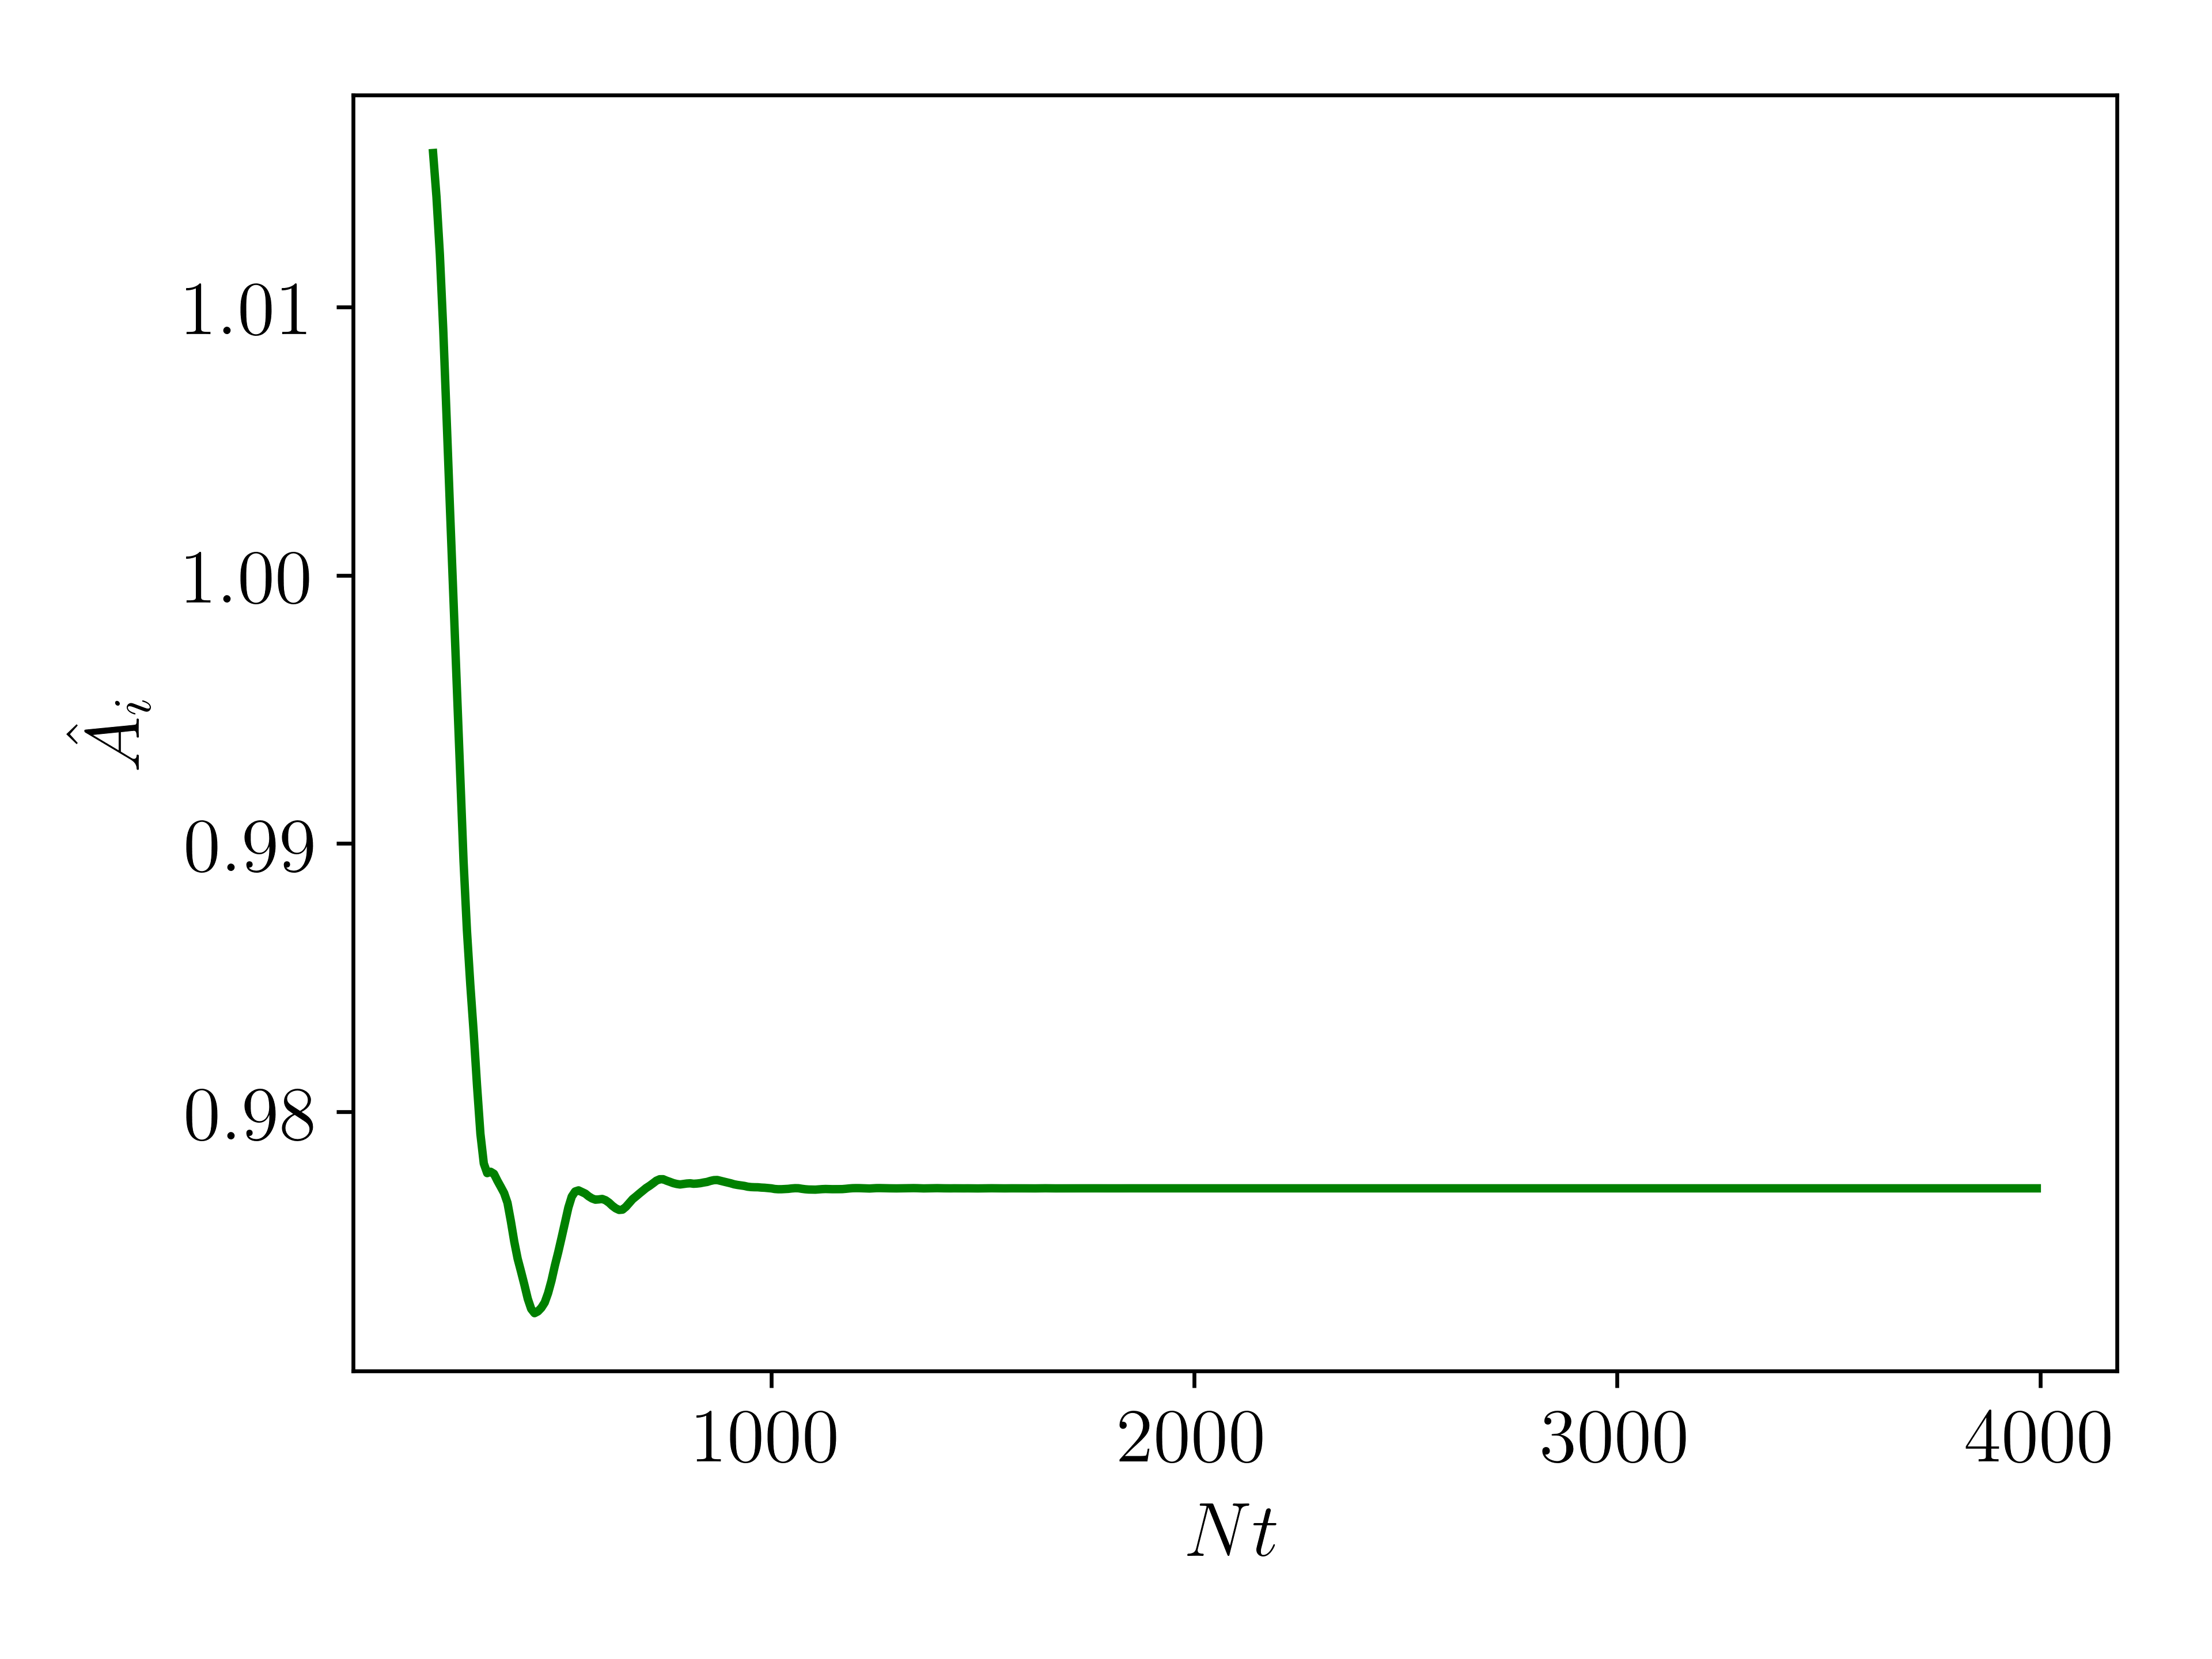
\includegraphics[width=\columnwidth]{plots/lin_amps.png}
    \caption{Amplitude of excited wave over time in weak forcing simulation,
    computed using \autoref{eq:ahat_def}. $\hat{A}(t) = 1$ corresponds to
    perfect agreement with the analytical estimate. After an initial transient
    phase, we observe great agreement with \autoref{eq:uz_lin}, and in
    particular $\hat{A}(t)$ asymptotes to a constant value, implying continuous
    excitation of identical IGW.}\label{fig:lin_amps}
\end{figure}

A second prediction of the analytical theory is that $S(z, t)$ should be
spatially flat between the forcing and damping zone(\autoref{eq:S_def}). We make
may a slightly more accurate estimate of $S_1$ the flux carried in the IGW by
directly substituting $\vec{u}_1$ into \autoref{eq:S_def}. Calling this estimate
$S_1$, we may then measure the agreement of our simulation with analytical
expectation by computing
\begin{equation}
    \hat{S}(z, t) \equiv \frac{\int\limits_0^{L_x}\rho u_xu_z\;\mathrm{d}x}{
        \int\limits_{0}^{L_x} \rho_0 u_{1x}u_{1z}\;\mathrm{d}x}.
        \label{eq:shat_def}
\end{equation}
For our weak forcing simulation, $\hat{S} = 1$ is expected between $z_0, z_T$,
and indeed we observe agreement with this in \autoref{fig:lin_fluxes}.
\begin{figure}[t]
    \centering
    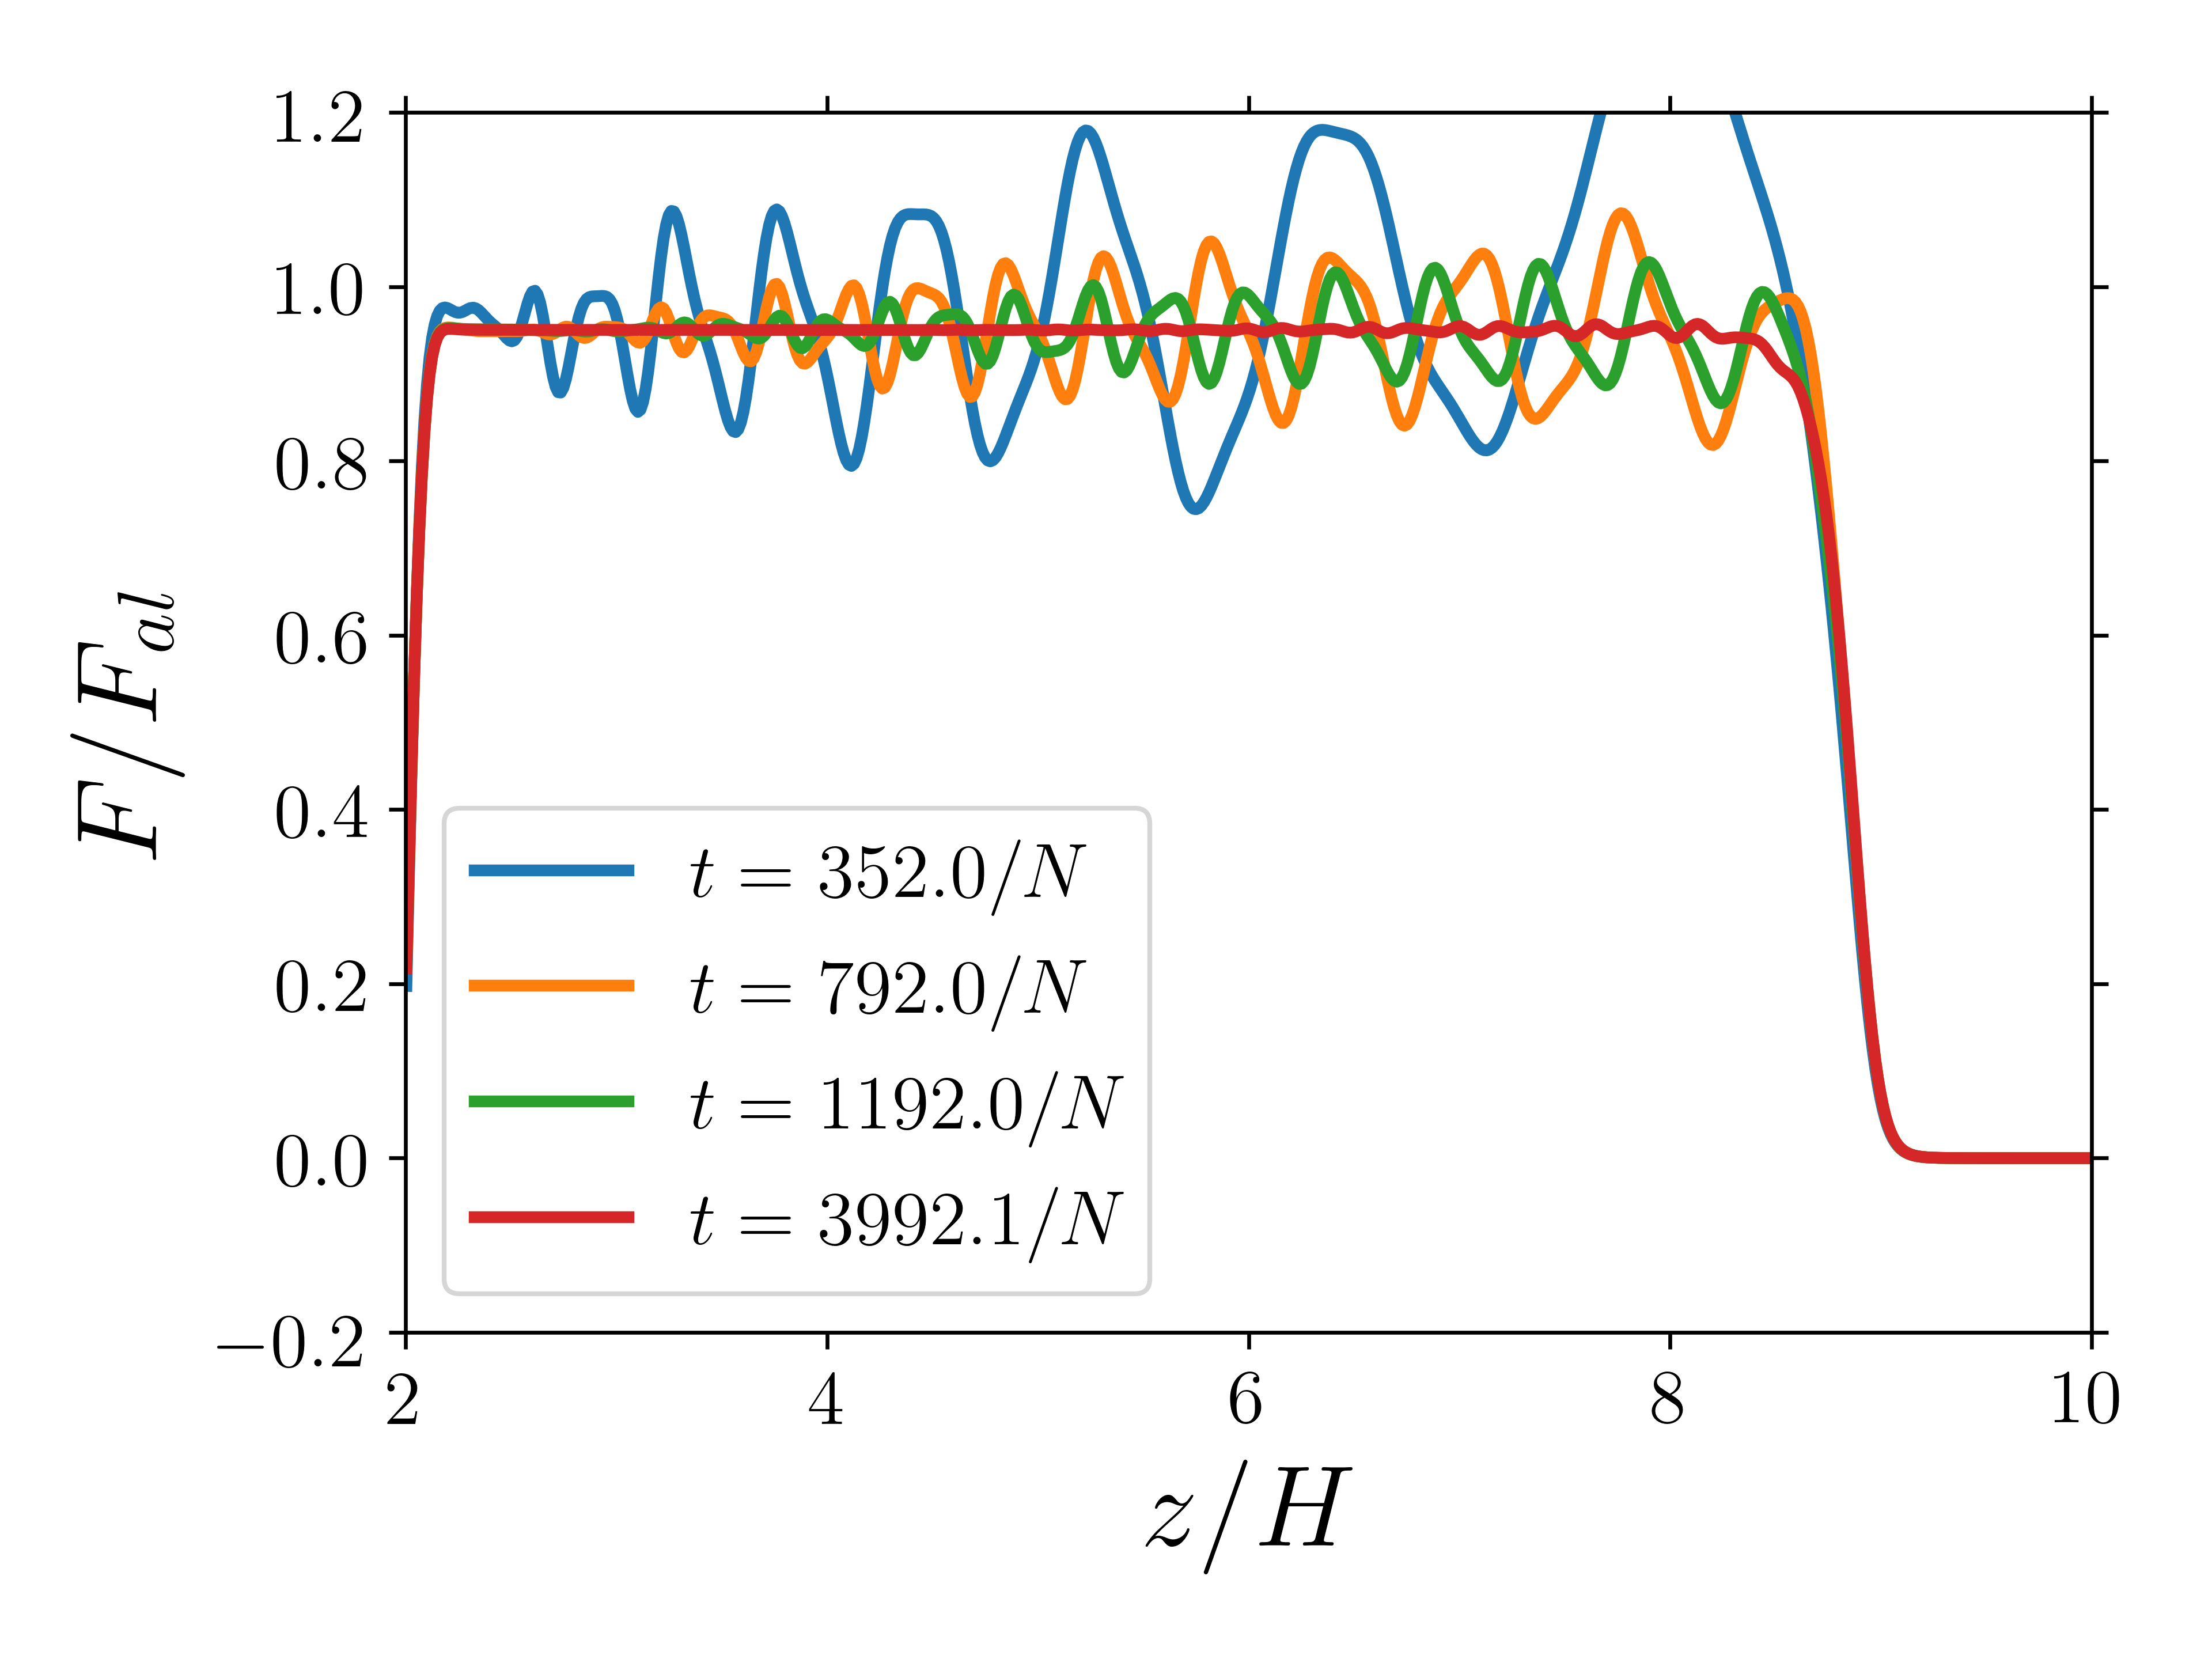
\includegraphics[width=\columnwidth]{plots/lin_fluxes.png}
    \caption{\autoref{eq:shat_def} as a function of $z$ at select times $t$. As
    initial transients die out, $\hat{S}(z, t) = 1$ to very good agreement below
    $z \lesssim z_T = 9.5H$. The flux excited in the forcing zone is transported
    without loss to the top of the domain, where it is dissipated by the damping
    layer (see \autoref{ss:damping}) without reflection.}\label{fig:lin_fluxes}
\end{figure}

\section{Internal Gravity Waves: Nonlinear Simulation}\label{s:sim}

To perform simulations of wave breaking phenomena, we use the same values as
\autoref{ss:numerics} except for $F, \nu$. In particular, we choose $F$ such
that $\vec{k}_1 \cdot \vec{\xi} = 0.1$ in the forcing zone, which implies
$\vec{k}_1 \cdot \vec{\xi}$ is exceeded before $z_T$ the upper damping zone.
The dissipation parameter $\nu$ was varied across the various simulations. To
quantify $\nu$, we define Reynolds number
\begin{equation}
    \mathrm{Re} = \frac{LU}{\nu} \equiv \frac{\omega_1}{\nu k_{1z}^2}.
        \label{eq:re_def}
\end{equation}
A table of our simulation viscosities can be found in \autoref{tab:params}.
\begin{table*}
    \centering
    \begin{tabular}{l c c c}
        Name & Resolution & $\mathrm{Re}$ & $z$ spectral basis\\\bottomrule
        \texttt{0p5\_hres} & $512 \times 2048$ & $2048$ & Fourier\\
        \texttt{0p5\_shres} & $1024 \times 4096$ & $2048$ & Fourier\\
        \texttt{1\_hres} & $512 \times 2048$ & $1024$ & Fourier\\
        \texttt{1\_vhres} & $768 \times 3072$ & $1024$ & Fourier\\
        \texttt{2\_hres} & $512 \times 2048$ & $512$ & Fourier\\
        \texttt{3\_width} & $256 \times 1024$ & $341$ & Fourier\\
        \texttt{6\_masked} & $256 \times 1024$ & $512$ & Chebyshev\\
        \texttt{4\_masked} & $256 \times 1024$ & $341$ & Chebyshev\\
        \texttt{3\_masked} & $256 \times 1024$ & $205$ & Chebyshev\\
        \texttt{1\_masked} & $256 \times 1024$ & $146$ & Chebyshev\\
    \end{tabular}
    \caption{Table of simulation parameters. Note that $\mathrm{Re}$ is defined
    as in \autoref{eq:re_def}.}\label{tab:params}
\end{table*}

\subsection{Numerical Simulation Results}\label{ss:nl_ns}

A full video of our higher-resolution run at $N_x = 1024, N_z = 4096$ can be
found at\footnote{ http://www.princeton.edu/~lecoanet/data/breaking\_wave.mov}.
Slices of $\bar{U}, \hat{S}$ across $z$ at various times $t$ are shown in
\autoref{fig:nl_fluxes}. While the behavior of $\bar{U}$ seems to conform
qualitatively with the predictions of \autoref{ss:crit_layer}, the behavior of
$\hat{S}$ exhibits two salient features: (i) the incident flux seems to fluctuate
greatly with time, and (ii) there seems to be a small transmitted feature at many
of the later times. We will discuss further these features in
\autoref{ss:reflectivity}, after first analyzing the propagation of the critical
layer.
\begin{figure}[t]
    \centering
    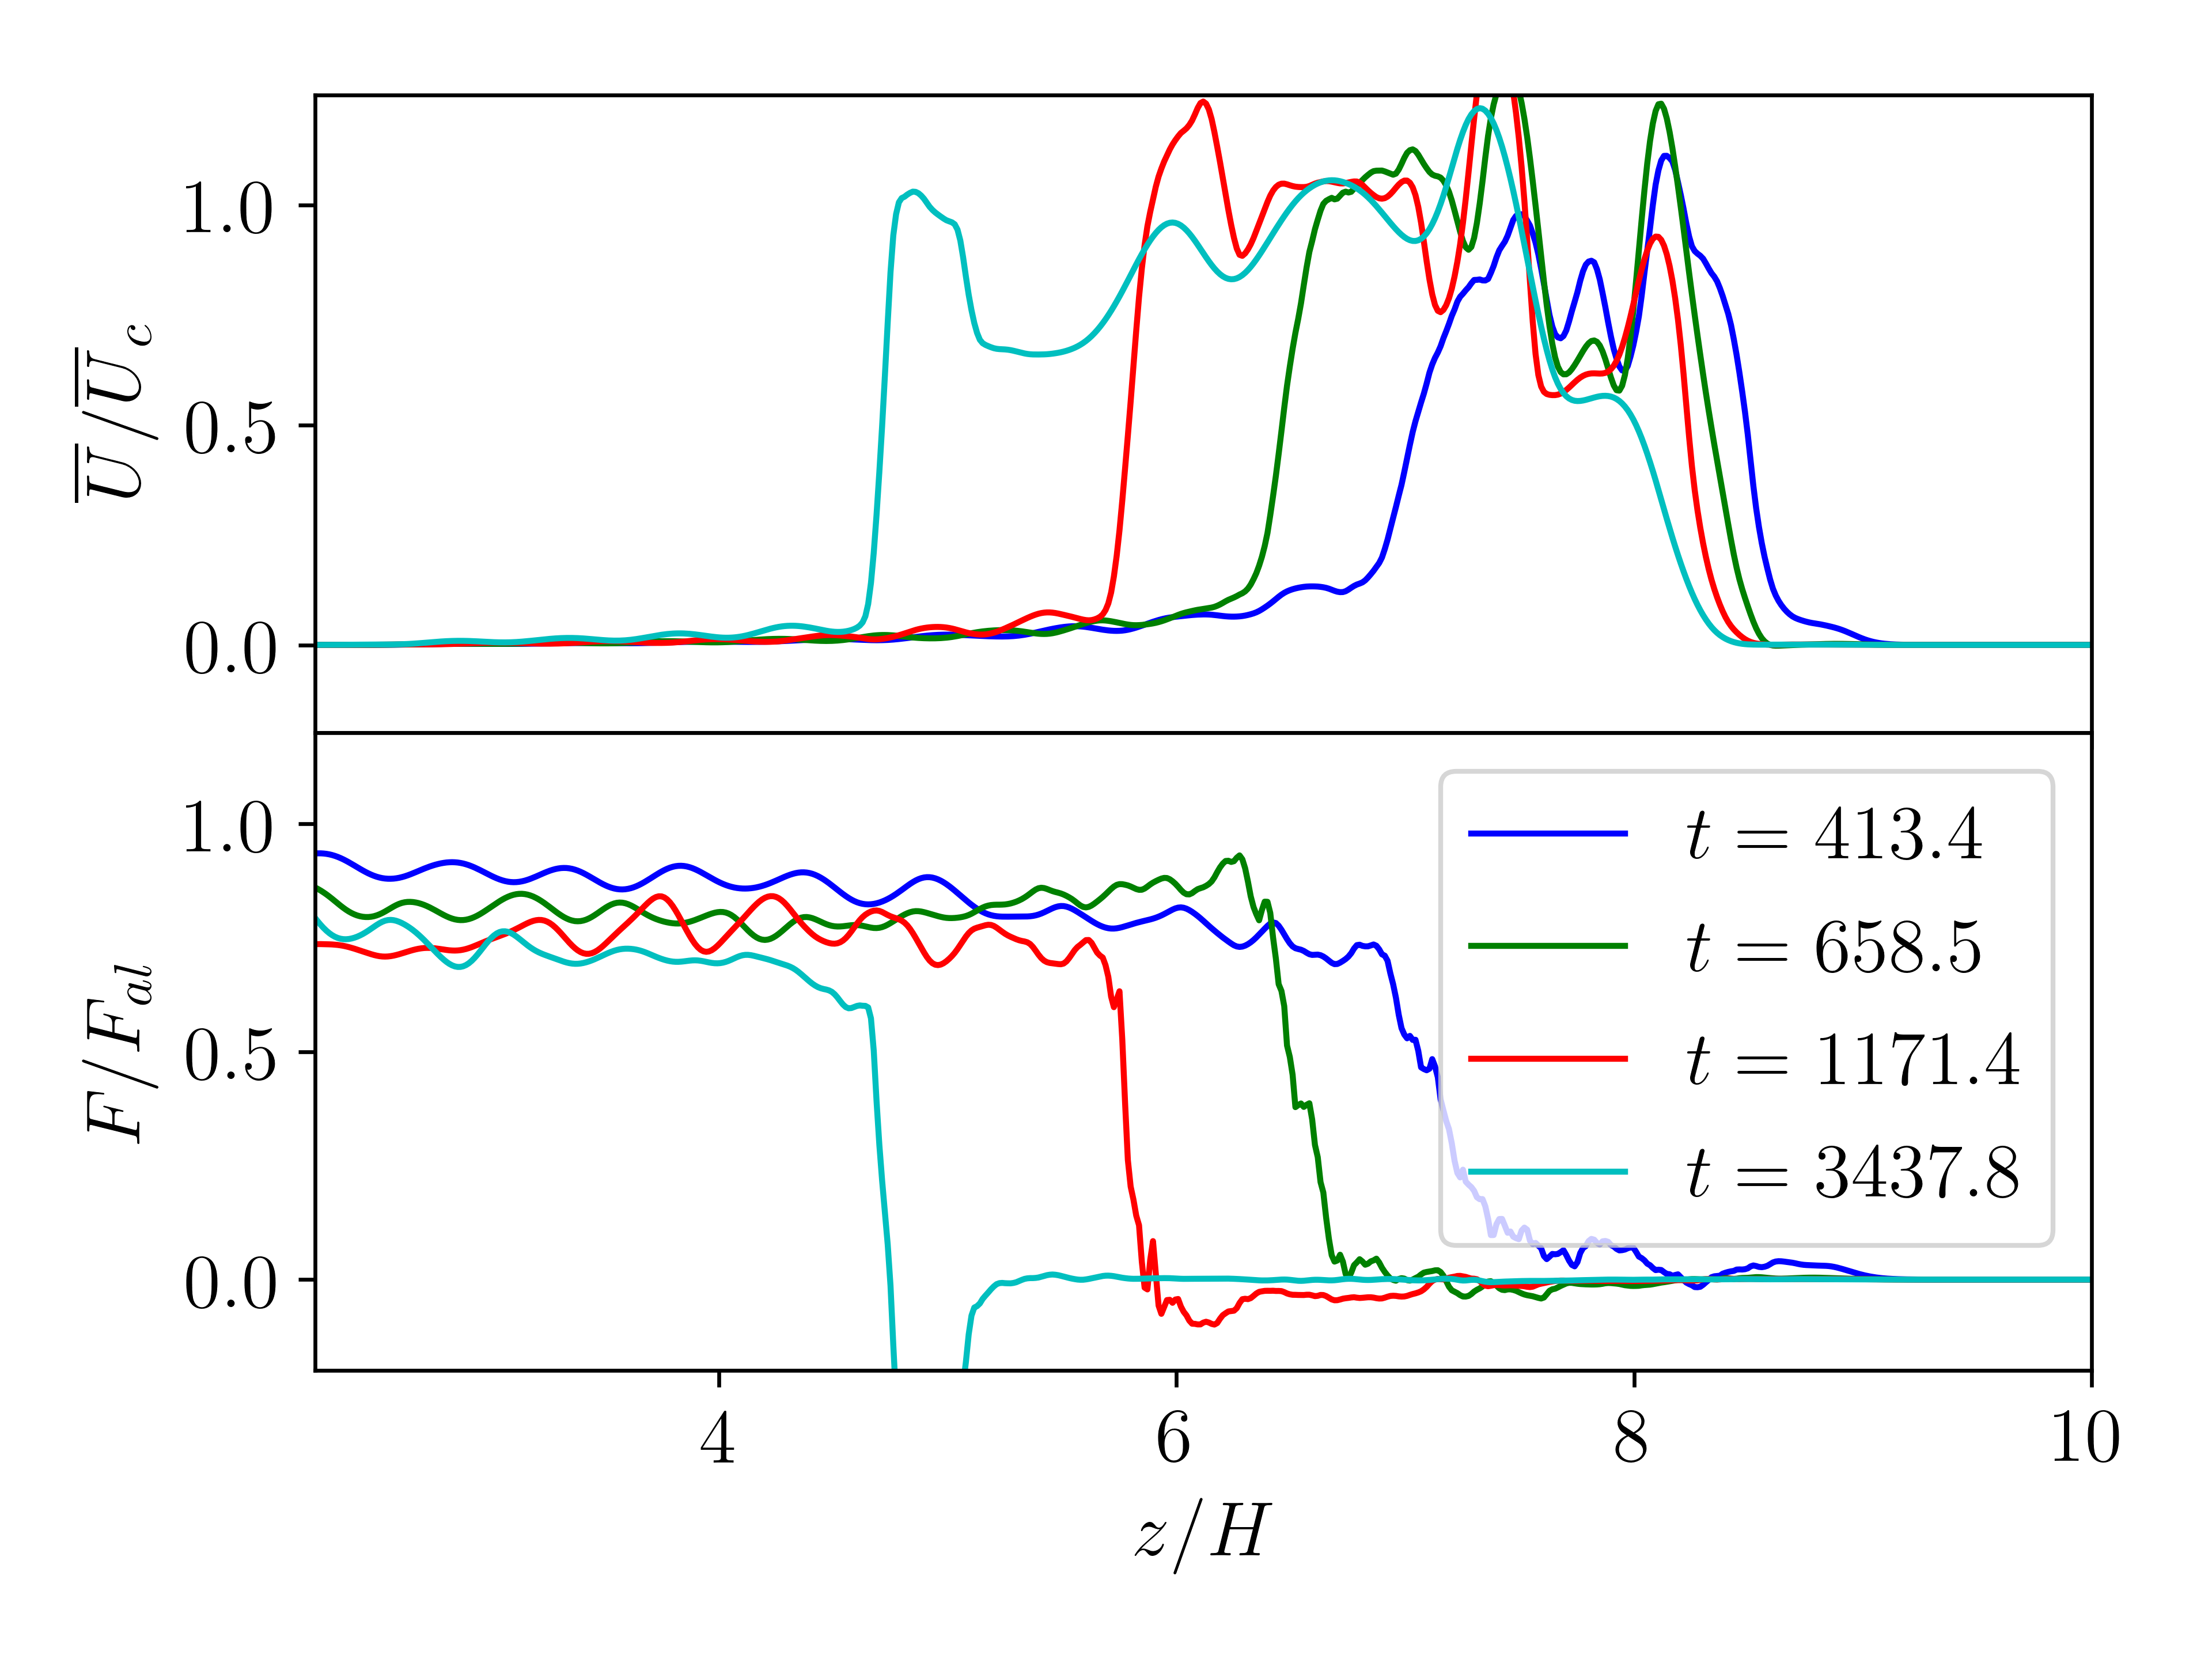
\includegraphics[width=\columnwidth]{plots/nl_fluxes.png}
    \caption{Plot of $\bar{U}(z, t)$ and $\hat{S}(z, t)$ respectively at various
    times over $z$. $\bar{U}, \hat{S}$ follow their definitions in
    \autoref{eq:mean_flow} and \autoref{eq:shat_def}. The values are extracted
    from run \texttt{0p5\_shres}. $\bar{U}$ is given
    in units of $c_{ph, x} = \frac{\omega_1}{k_{1x}}$ the critical layer flow
    velocity (see \autoref{ss:crit_layer}). The propagation of the critical
    layer towards lower $z$ and sharp deposition of $S$ at the critical layer
    are evident.}\label{fig:nl_fluxes}
\end{figure}

\subsection{Propagating Critical Layer}

For the simulation shown in \autoref{fig:nl_fluxes}, we may analyze the location
of the critical layer. As the simulations are very noisy, we define the location
of the critical layer to be
\begin{align}
    z_{c, \min} &= \argmin_z \z{z: S(z) < 0.3S_0},\nonumber\\
    z_{c, \max} &= \argmax_z \z{z: S(z) > 0.3S_0},\nonumber\\
    z_c &\equiv \frac{z_{c, \min} + z_{c, \max}}{2}.\label{eq:zc_def}
\end{align}
This was found to a relatively stable estimator of the critical layer location.
Other estimators were used and do not significantly change the results of the
analysis.

The evolution of $z_c$ is described by ODE \autoref{eq:zc_anal}, and in the
limit $\Delta S(t) = \Delta S$ we obtained closed-form solution
\autoref{eq:zc_sol}. To estimate $\Delta S(t)$ from the data, we defined:
\begin{align}
    S_{<}(t) &= \ev{S(z)}_{z \in [z_c - \Delta z - H, z_c - \Delta z]}
        ,\label{eq:sbelow_def}\\
    S_>(t) &= \ev{\z{S(z): S(z) < 0}}_{z \in [z_c, z_c + \Delta z]},
        \label{eq:sabove_def},\\
    \Delta S(t) &\equiv S_>(t) - S_{<}(t).\label{eq:ds_def}
\end{align}
$\ev{\dots}_{z \in [z_a, z_b]}$ denotes averaging over interval $[z_a, z_b]$.
We average over an interval of length $H = \frac{2\pi}{k_{1z}}$ a full vertical
wavelength. The offset $\Delta z$ is set by the observation that the critical
layer's width is limited by $\mathrm{Ri} \lesssim 1$, translating to a critical
layer width of $\sim \frac{1}{k_{1z}}$. Here, we found $\Delta z =
\frac{3}{k_z}$ was necessary to be sufficiently offset from strong fluctuations
near the critical layer.

Since the transmission feature can be seen in \autoref{fig:nl_fluxes} to
attenuate rather quickly and is indeed rather weak, it is difficult to establish
the correct interval to average over; we use the observation that $S(z) < 0$
only for a small interval for $z$ to select the interval length implicitly.

Finally, we may plot the observed $z_c$ from data against two simple predictors:
(i) integration of \autoref{eq:zc_anal} using the measured $\Delta S(t)$, and
(ii) substituting the time-averaged $\ev{\Delta S}_t$ into \autoref{eq:zc_sol}.
Since $z_c(t)$ is both stable and less well-defined at early times (when the
critical layer is thick and transient behavior is still strong), we instead
integrate backwards from the end of the simulation, using $z_c(t_f)$ as initial
condition. The resulting predictors are depicted in \autoref{fig:nl_front}. The
good agreement between the evolution of $z_c(t)$ and its estimate via $\Delta
S(t)$ and \autoref{eq:zc_anal} are noteworthy. Further of interest is the
discrepancy between the time-averaged predictor and the data. The general
agreement clearly demonstrates $\Delta S < S_1$ and that incomplete absorption
is observed. Moreover, its significant underprediction of critical layer motion
at early times contrasts with its comparatively satisfactory prediction at later
times to indicate that $\Delta S(t)$ must vary significantly over time. Both of
these observations indicate a careful characterization of reflectivity is
necessary.

\begin{figure}[t]
    \centering
    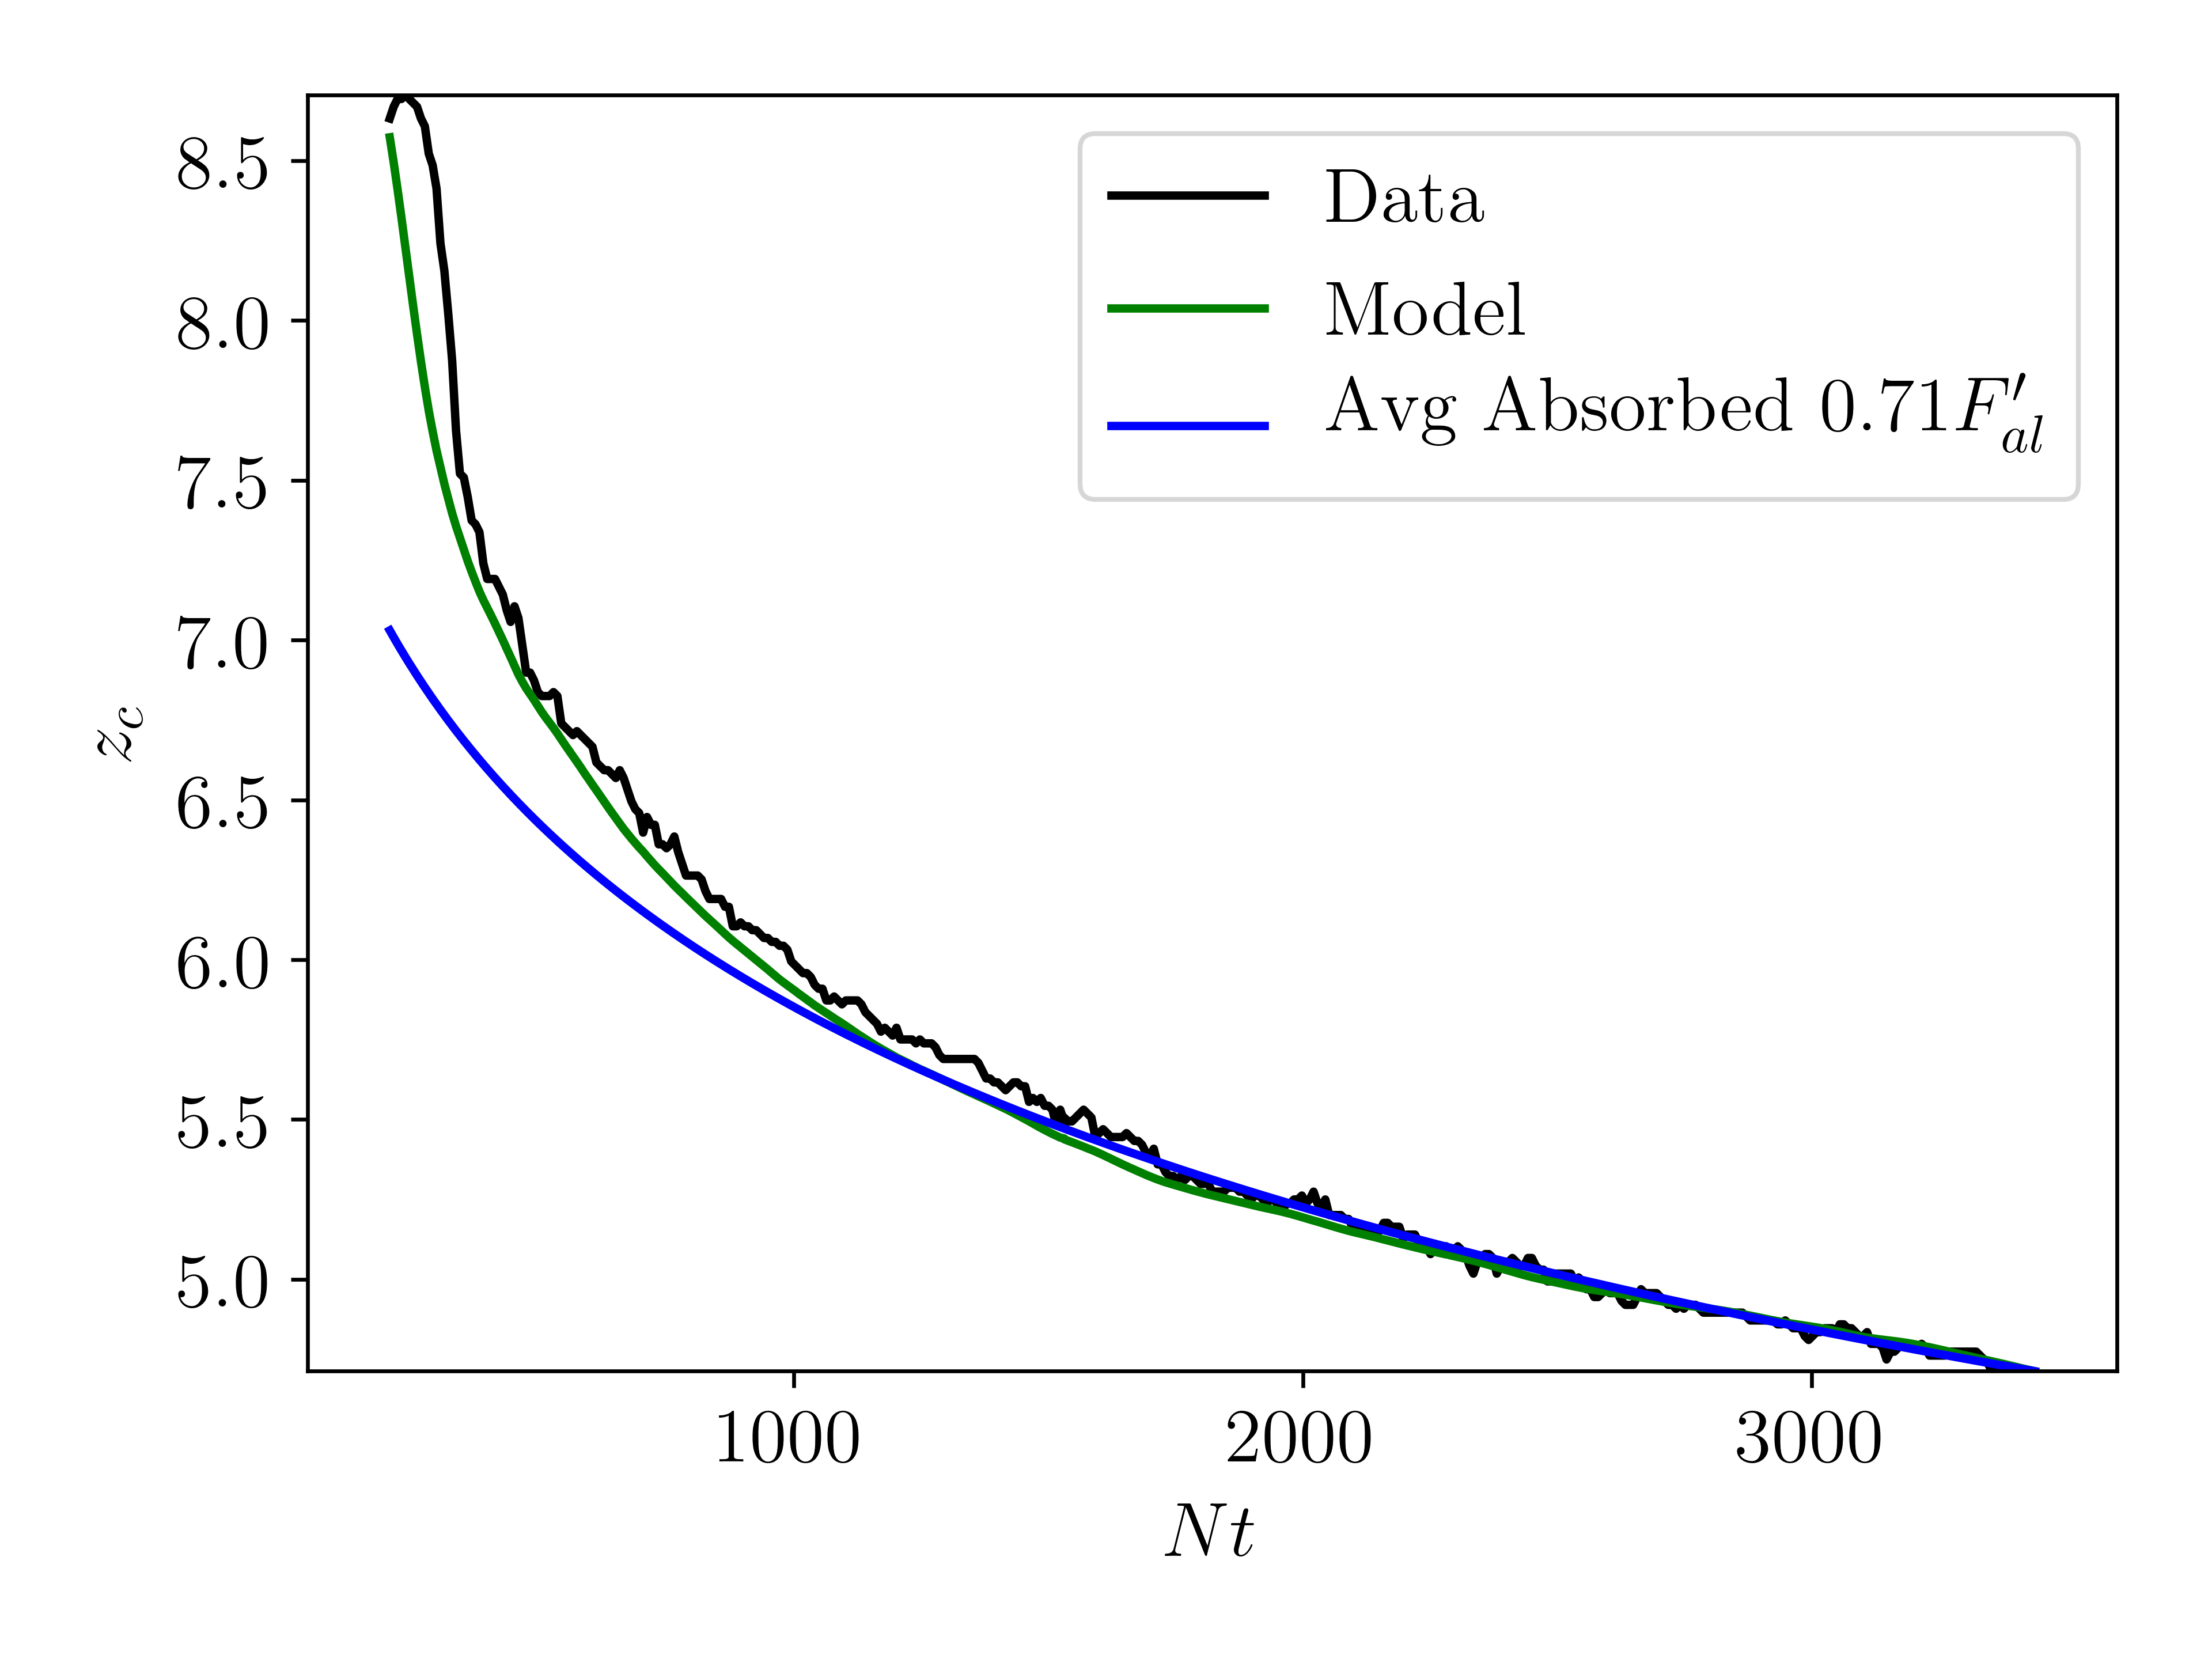
\includegraphics[width=\columnwidth]{plots/nl_front.png}
    \caption{Propagation of the critical layer over time. Shown are (black)
    $z_c(t)$ from simulation data, (green) predictor of $z_c(t)$ using direct
    integration of \autoref{eq:zc_anal} for $\Delta S(t)$ measured from
    simulation data (described in \autoref{eq:ds_def}) and (blue) direct
    substitution of time-averaged $\ev{\Delta S(t)}_t$ into
    \autoref{eq:zc_sol}. Predictors use the end of the simulation as initial
    conditions and integrate backwards, as $z_c$ is less well-defined at early
    times. The agreement of the directly-integrated predictor with the data
    shows \autoref{eq:zc_anal} is a good description of the evolution of $z_c$.
    The the poorer but qualitatively correct agreement of the time-averaged
    predictor with the data shows both that $\Delta S(t) \neq S_1$ and that
    $\Delta S(t)$ likely has some very real variation with
    time.}\label{fig:nl_front}
\end{figure}

\subsection{Kelvin-Helmholtz Instability and Critical Layer Width}

The observation of reflected/transmitted waves is in accordange with previous
studies as discussed in \autoref{ss:wave_breaking}. Many studies have shown that
a local Richardson number $\mathrm{Ri} \sim 1/4$ corresponds to the onset of
reflectivity. This agrees with the observed Kelvin-Helmholtz instability in our
simulations [TODO image]. To verify that the critical layer's width is bound
from below by Kelvin-Helmholtz instabilities, we decided to compute a
$\mathrm{Ri}$ within the critical layer.

Since fluid instabilities are local, $\mathrm{Ri}$ must be measured in the
immediate vicinity of a fluid parcel. Thus, we first assign an $\mathrm{Ri}$ for
every $x$ in the critical layer, then take the median as $\mathrm{Ri}$ for the
entire layer. To avoid noisiness, the local $\mathrm{Ri}$ is computed using the
vertical distance over which the local $u_x$ increases from $0.3 \times$ its
critical value to its critical value. This can be written
\begin{align}
    z_{u, \min}(x, t) &= \argmin_\zeta
        \z{z: u_x(x, \zeta, t) > 0.3\bar{U}_c},\nonumber\\
    z_{u, \max}(x, t) &= \argmax
        \zeta \z{z: u_x(x, \zeta, t) < \bar{U}_c},\nonumber\\
    \mathrm{Ri}(t) &\equiv
        \med_x\p{\frac{N^2 \p{z_{u, \max} - z_{u, \min}}^2}{(0.7
            \bar{U}_c)^2}}.\label{ss:ri_med_def}
\end{align}
To understand the variation in $\mathrm{Ri}$ over $x$, we can also plot using
the minimum over $x$; the maximum is significantly noisier. Both of these are
shown in \autoref{fig:nl_f_ri}. The quick evolution of $\mathrm{Ri}$ to its
saturated value is reflective of the fact that IGW are \emph{anti-diffusive}.
This property is a simple consequence of the IGW dispersion relation
\autoref{eq:disp_rel}, which is approximately $\omega k_z \approx Nk_x$ such
that as an IGW propagates into a shear flow, $\omega$ decreases and $k_z$
increases, enhancing dissipation. Dissipation in a momentum-conserving fluid
then corresponds to further mean flow acceleration.
\begin{figure}[t]
    \centering
    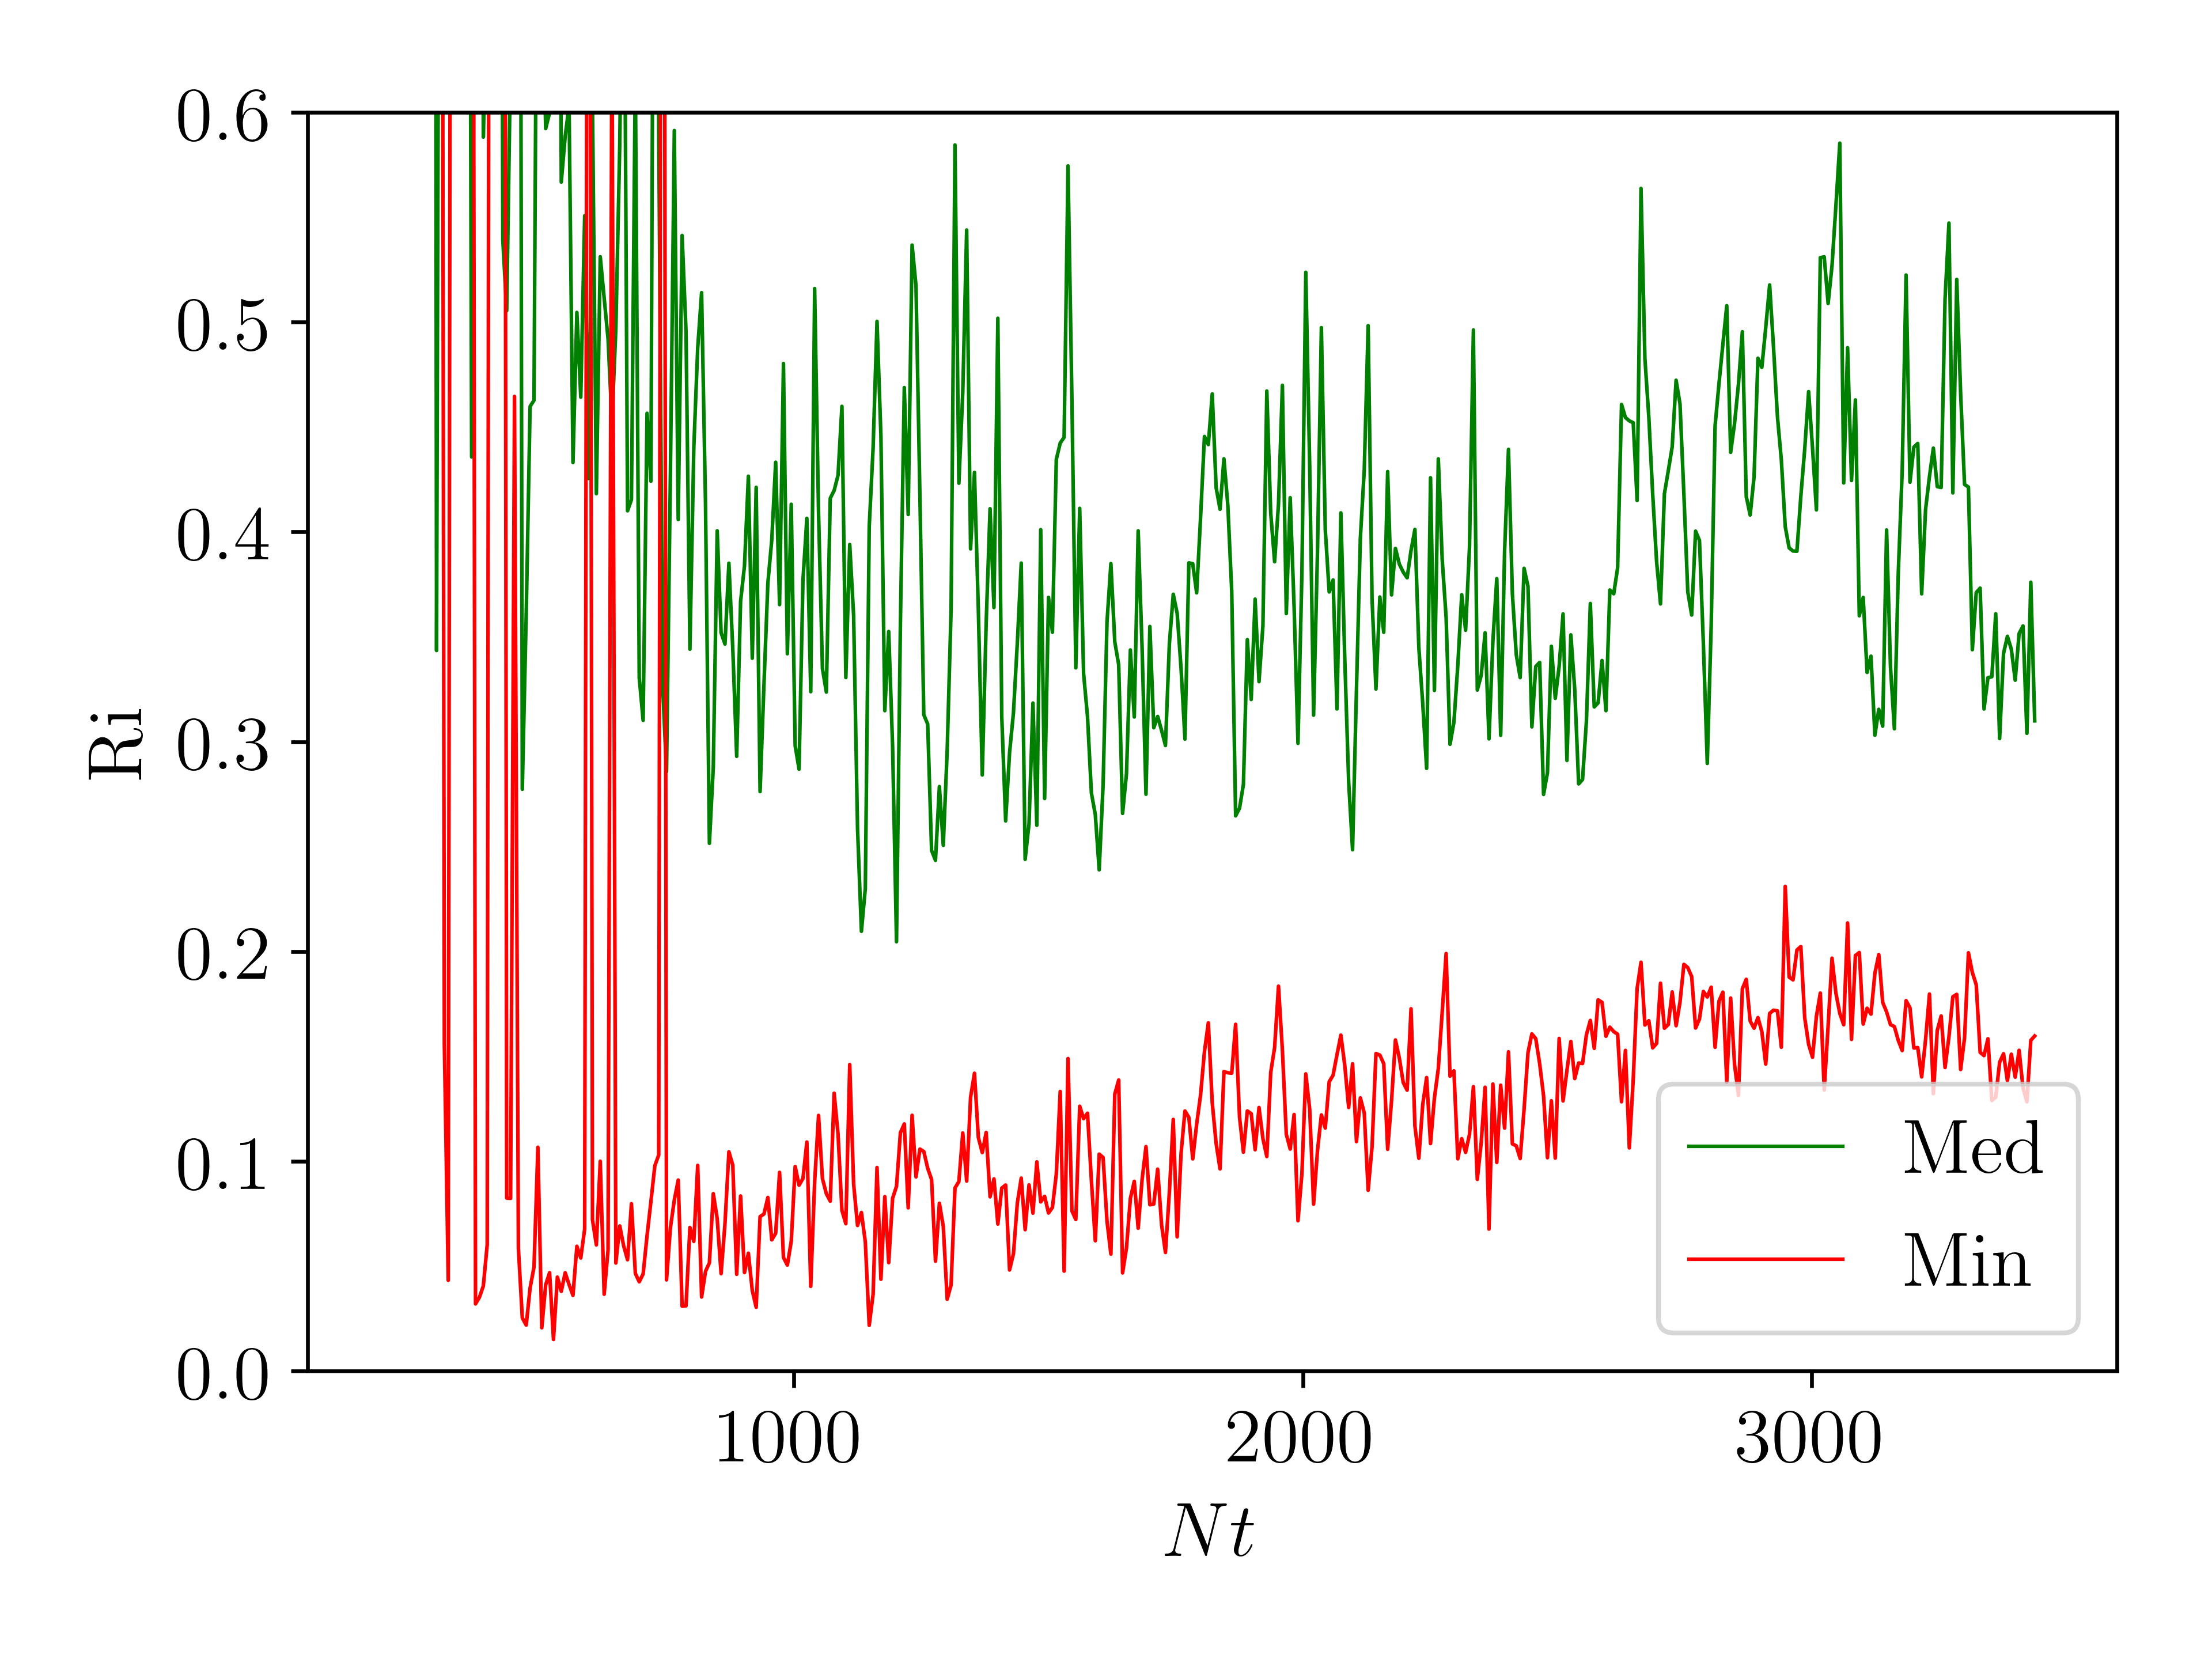
\includegraphics[width=\columnwidth]{plots/nl_f_ri.png}
    \caption{Local Richardson number of the flow at the critical layer over time
    as defined in \autoref{ss:ri_med_def}. Dotted red lines demarcate the
    minimum and maximum of $\mathrm{Ri}$ over $x$ instead of the median. These
    numbers effectively measure the mean and spread in width of the critical
    layer over $x$. Note that $\mathrm{Ri} \lesssim \frac{1}{4}$ corresponds
    to Kelvin-Helmholtz instability, so this plot suggests the critical layer
    width roughly saturates the lower bound from the Kelvin-Helmholtz
    instability after an initial transient phase.}\label{fig:nl_f_ri}
\end{figure}

\subsection{Non-absorption at Critical Layer}\label{ss:reflectivity}

We identify two instances of non-absorptive behavior: (i), the presence of a
reflected wave with wave vector $\vec{k} = k_{1x}\hat{x} + k_{1z}\hat{z}$, and
(ii) the amount of horizontal momentum flux $S$ reflected off the critical
layer.

To measure the reflected wave amplitude, we use almost the same definition
\autoref{eq:ahat_def} except using $-k_{1z} \to +k_{1z}$; call this estimated
$\hat{A}_r(t)$ the amplitude of the downwards-propagating reflected wave, and
call $\hat{A}_i(t)$ the upwards-propagating incident wave. To compute
$\hat{A}_r(t)$, we furthermore permit an arbitrary phase offset $\phi_r(t)$ at
each time $t$, since the phase of the reflected wave is unknown, unlike that of
the incident wave. We observe that the evolution of $\phi_r(t)$ is consistent
with the interpretation of a reflected wave, as it is well approximated by
$\pd{\phi_r}{t} \approx 2\pd{(k_{1z}z_c)}{t}$, consistent with a wave reflecting
off a moving boundary at $z_c$.

Since reflectivity depends sensitively on accurate measurements of $\hat{A}_i,
\hat{A}_r$, it is important \autoref{eq:ahat_def} identically not pick up
contributions between the two $k_{1x}\hat{x} \pm k_{1z}\hat{z}$ modes, as we
argued earlier. The integral for $\hat{A}_r$ is also performed over $z \in [z_0
+ 3\sigma, z_0 + 3\sigma + H]$. Since in general $\hat{A}_i(t), \hat{A}_r(t)$
are functions of time, we must measure reflectivity accounting for propagation
time between the measurement zone and the critical layer where the wave
reflects. For some
\begin{equation}
    \delta t(t) \approx \frac{z_c(t) - z_0 + 3\sigma + H/2}{c_{ph, z}},
        \label{eq:dt_def}
\end{equation}
an incident wave measured at $t - \delta t$ reflects at $t$ and is re-measured
as a reflected wave at $t + \delta t$. The choice of vertical phase velocity
instead of group velocity is necessary to good results, and a possible
explanation is provided in \autoref{ss:modes}. We can then define the amplitude
reflectivity
\begin{equation}
    \mathcal{R}_A(t) \equiv \frac{\hat{A}_r(t - \delta t)}{\hat{A}_i(t +
        \delta t)}.\label{eq:Ra_def}
\end{equation}
Since in general $\delta t$ can take on arbitrary values while $\hat{A}_i,
\hat{A}_r$ are sampled at discrete timesteps set by our simulation output, we
evaluate $\hat{A}_i, \hat{A}_r$ using a simple linear interpolation to
intermediate times.

To measure the reflected horizontal momentum flux, we recall from our linear
simulations described in \autoref{ss:lin_ns} that we are able to accurately
predict the incident flux from the incident wave amplitude. Thus, we write for
incident flux
\begin{equation}
    S_i(t) \equiv \ev{\rho u_{1x} u_{1z}}_x\hat{A}_i^2(t).
\end{equation}
But then, since we already have $\Delta S(t), S_>(t)$ jump and transmitted flux
across the critical layer at time $t$ respectively, we can immediately write
down the reflected flux
\begin{equation}
    S_d(t) = S_i(t - \delta t) + \Delta S(t) - S_>(t).
\end{equation}
$\delta t$ is still \autoref{eq:dt_def}; propagation time between $z_c$ and $z_c
- 3/k_z - H/2$ the center averaging zone was ignored at the level of accuracy of
the study. Then we can define flux reflectivity and transmissivity coefficients
\begin{align}
    \mathcal{R}_S(t) &\equiv -\frac{S_d(t)}{S_i(t - \delta t)},&
    \mathcal{T}_S(t) &\equiv -\frac{S_>(t)}{S_i(t - \delta t)}.
        \label{eq:srefl_def}
\end{align}

The measurements of $\hat{A}_i, \hat{A}_r, S_i, \Delta S, S_d, S_>$ are given in
\autoref{fig:nl_f_amps}. The oscillations in $\hat{A}_i, S_i$ are evident and
neatly correspond to oscillations in $A_d, S_d$ respectively. We further analyze
these oscillations in \autoref{ss:modes}.

\begin{figure}[t]
    \centering
    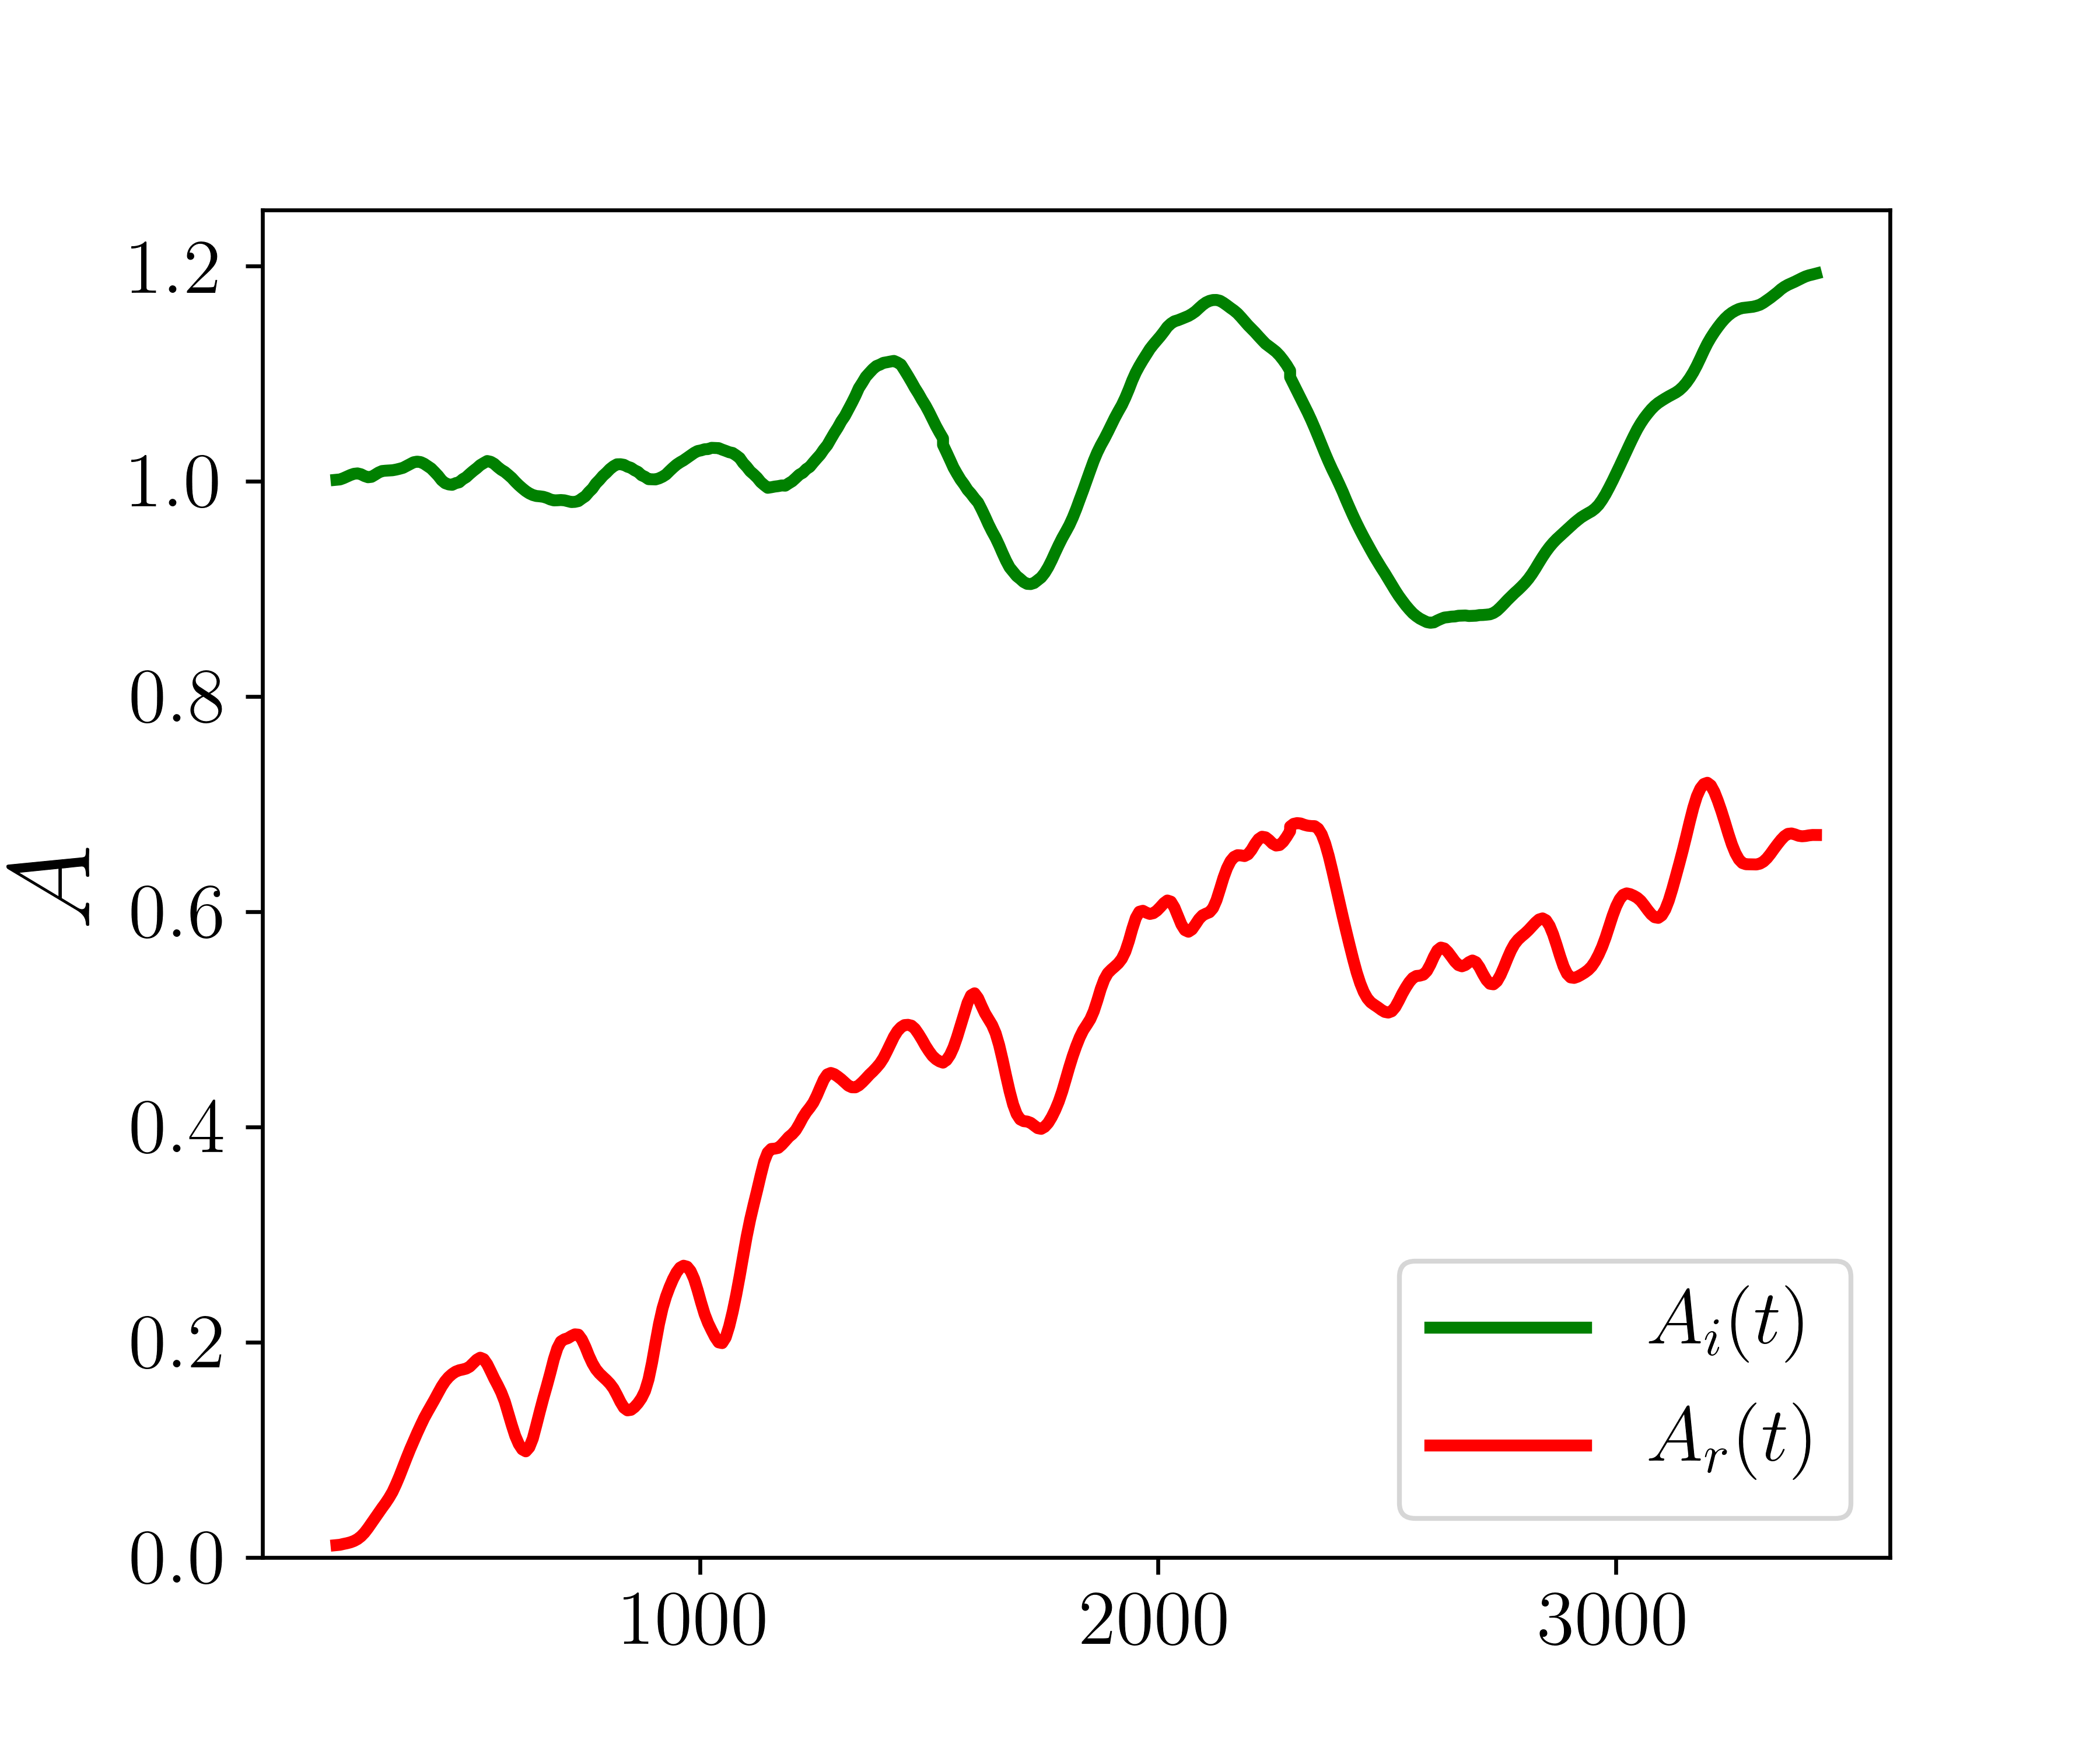
\includegraphics[width=\columnwidth]{plots/nl_f_amps.png}
    \caption{The top panel measures the incident wave amplitude $\hat{A}_i(t)$
    (green) and the downwards propagating wave amplitude $\hat{A}_r(t)$ (red)
    just above the forcing zone, normalized to the analytical estimate
    \autoref{eq:uz_lin}. $A_d \neq 0$ due to reflection off the critical layer.
    The bottom panel shows the behavior of three horizontal momentum fluxes over
    time, in units of the analytical estimate \autoref{eq:S_lin}: (blue) flux
    incident on the critical layer, (red) flux absorbed by the critical layer,
    and (black) flux transmitted through the critical layer. Note that no
    propagation time effects have been included in these plots.
    }\label{fig:nl_f_amps}
\end{figure}

Using these measured quantities, we may make plots of $\mathcal{R}_A^2,
\mathcal{R}_S, \mathcal{T}_S$, which are provided in \autoref{fig:nl_f_refl}. A
comparison between $\mathcal{R}_A^2$ and $\mathcal{R}_S$ is appropriate as $S
\propto A^2$. While less evident in the presented plot, a longer-duration
simulation at lower resolution confirms that the three quantities have reached
their asymptotic values after $t \gtrsim 1750/N$. An observation may be made
that in general $\mathcal{R}_S \geq \mathcal{R}_A^2$; this conforms to the
intuition that reflected flux consists of the simple reflected mode and higher
order modes as well.

\begin{figure}[t]
    \centering
    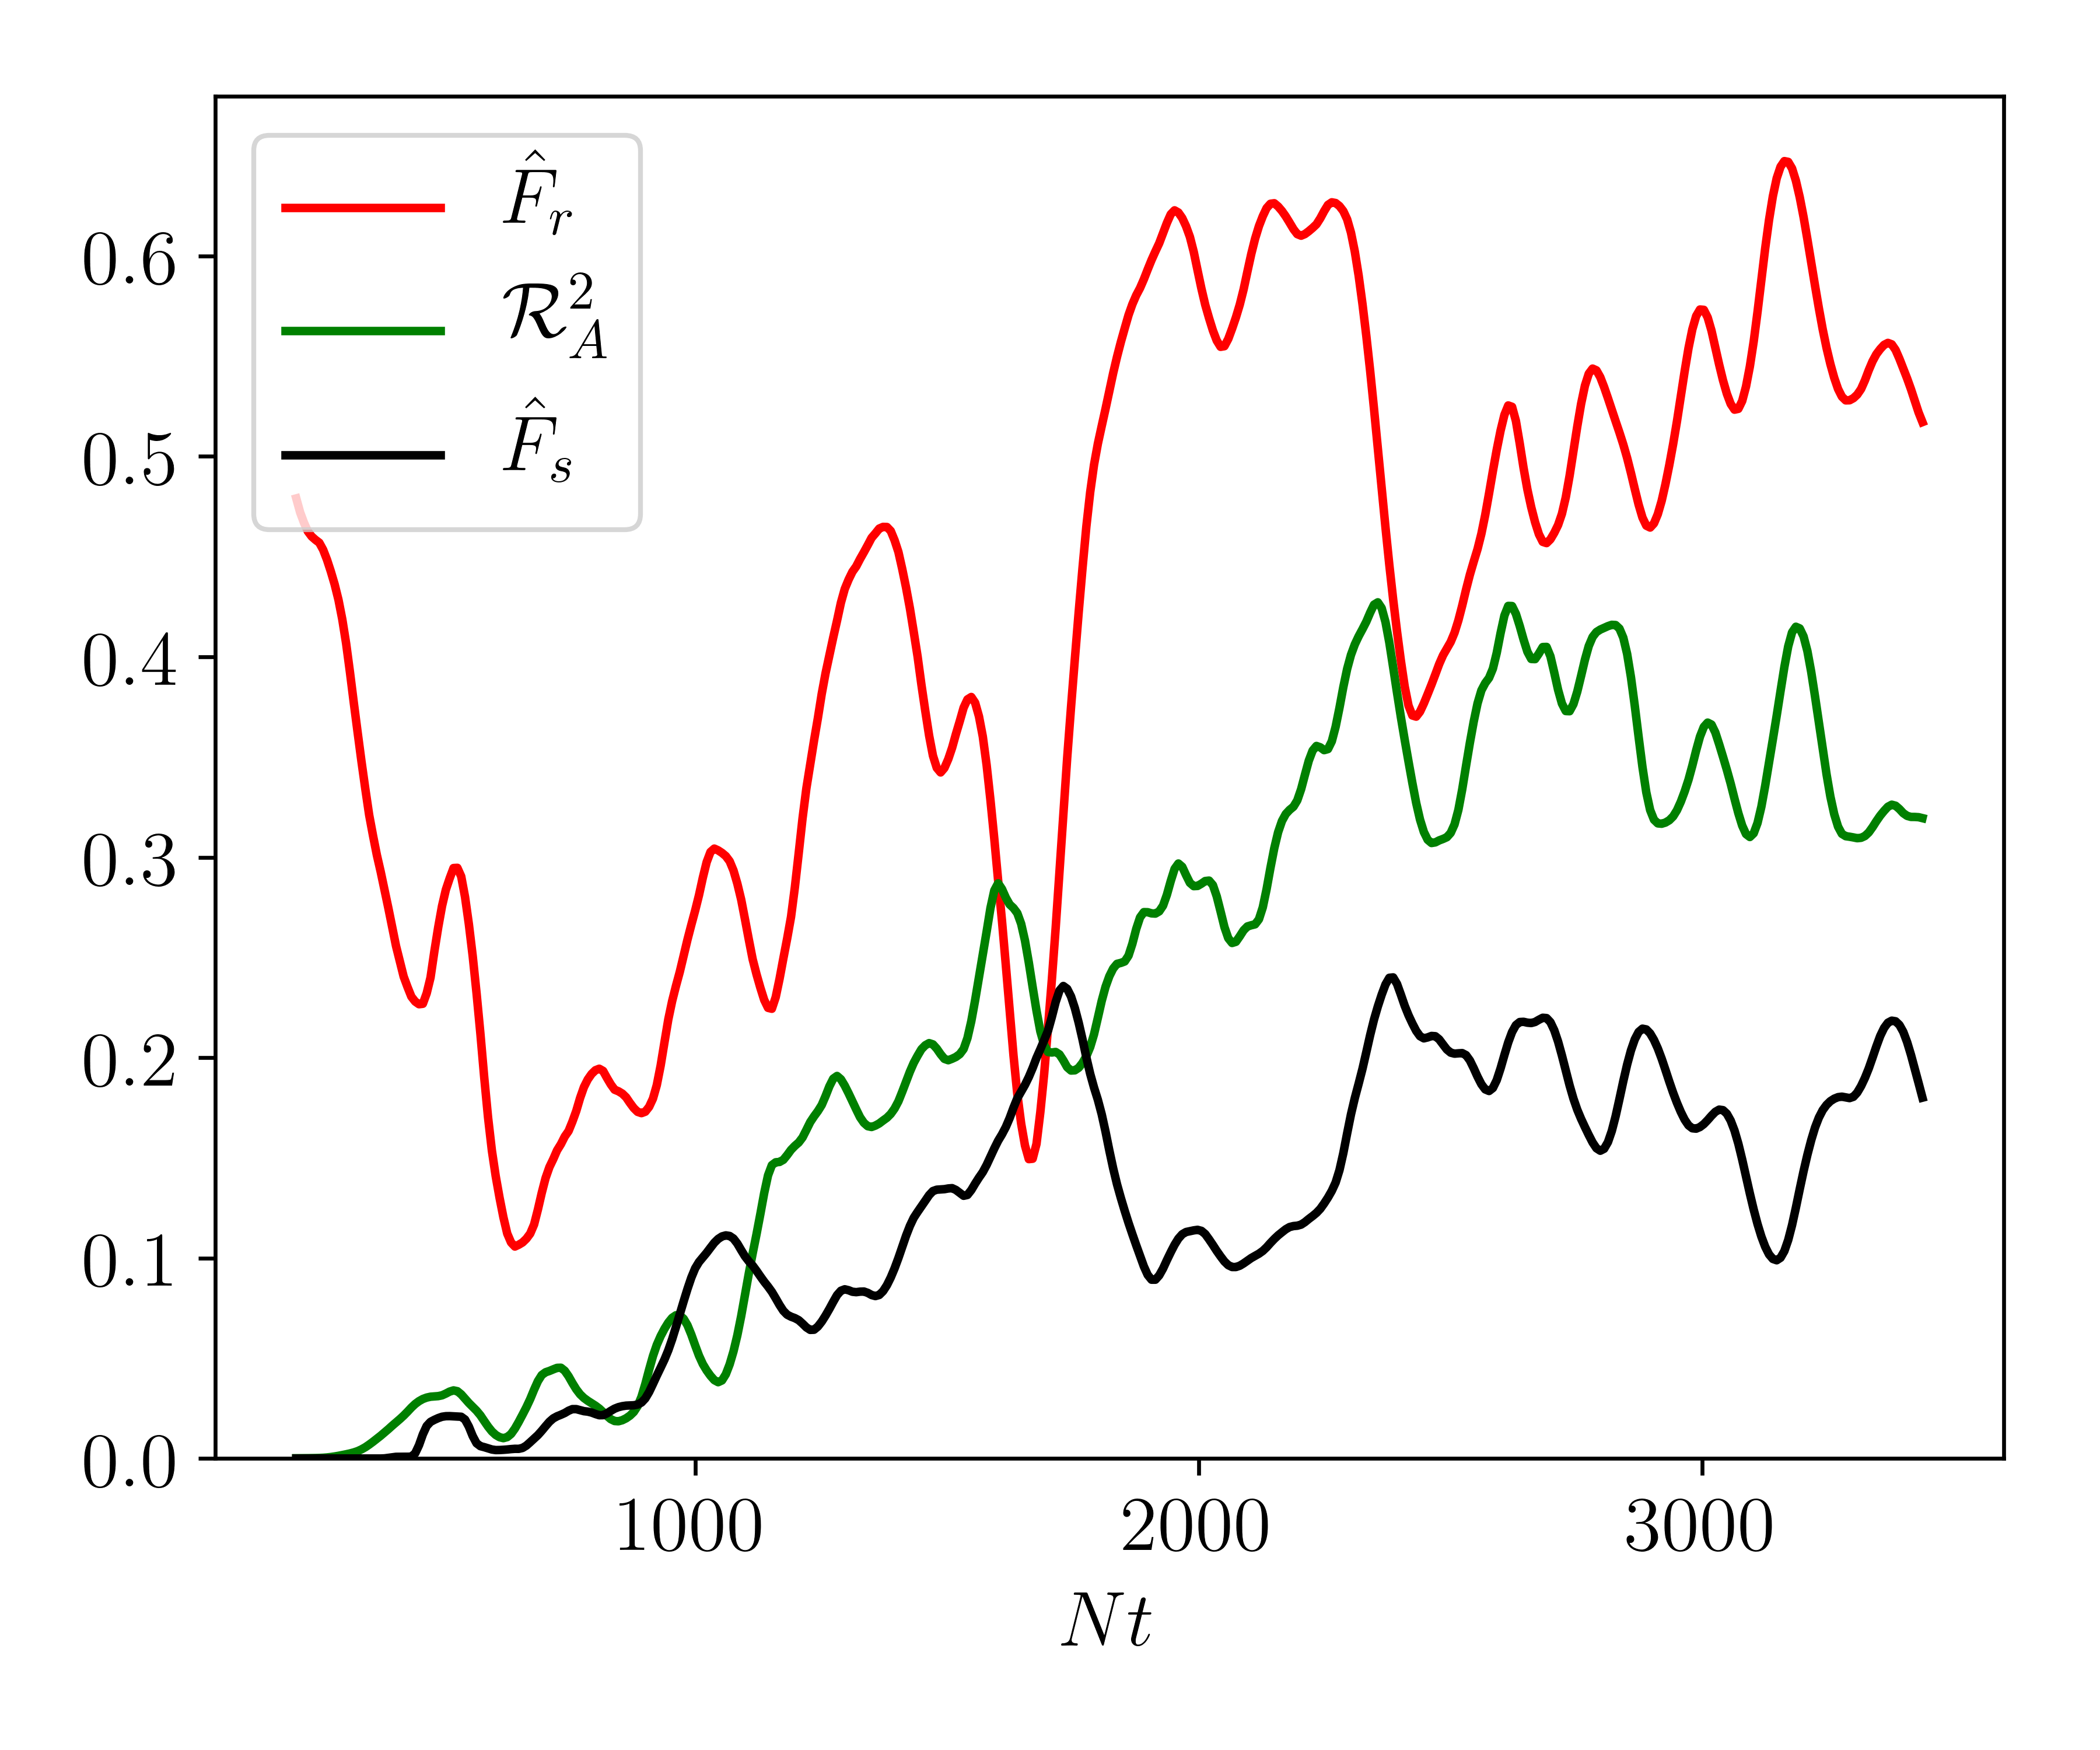
\includegraphics[width=\columnwidth]{plots/nl_f_refl.png}
    \caption{Reflectivity and transmittivity coefficients for flux and
    amplitude-squared as described by \autoref{eq:Ra_def} and
    \autoref{eq:srefl_def} respectively. The coefficients seem to become
    comparatively stable past about $t = 1750/N$, indicating that an asymptotic
    value may have been reached.}\label{fig:nl_f_refl}
\end{figure}

Finally, we may be interested in the power spectrum of the transmitted
horizontal momentum flux. Define:
\begin{align}
    \tilde{S}_>(k_x, t) = \abs{
        \int\limits_0^{L_x} e^{ik_xx}\hat{S}_>(x, z_c - \Delta z, t)\;\mathrm{d}x}
            \label{eq:sfft_above},\\
    \tilde{S}_<(k_x, t) = \abs{
        \int\limits_0^{L_x} e^{ik_xx}\hat{S}_<(x, z_c + \Delta z, t)\;\mathrm{d}x}.
            \label{eq:sfft_below}
\end{align}
These values are plotted in \autoref{fig:nl_fft}. Note that we expect
$\tilde{S}_<(0, t) = S_<(t) = S_i(t) + S_d(t)$ and the same for $\tilde{S}_>$.
This is rather accurate for $\tilde{S}_<$ but less so for $\tilde{S}_>$; this is
since $S_>(t)$ decays very rapidly above $z_c$. Note furthermore that at later
times, the transmitted flux increases, per expectation, and shifts towards
higher $k_x$. Repeating this plot at higher viscosities shows significantly
lower $\tilde{S}_>$, showing that the $k_x$ of the transmitted waves still
changes greatly at the highest $\mathrm{Re}$ we are able to probe. Finally, note
that the area under $\tilde{S}$ changes with time; this is okay since we are
measuring $S$ at constant position, and different $k_x$ components of $S$ will
translate at their separate group velocities.

\begin{figure}[t]
    \centering
    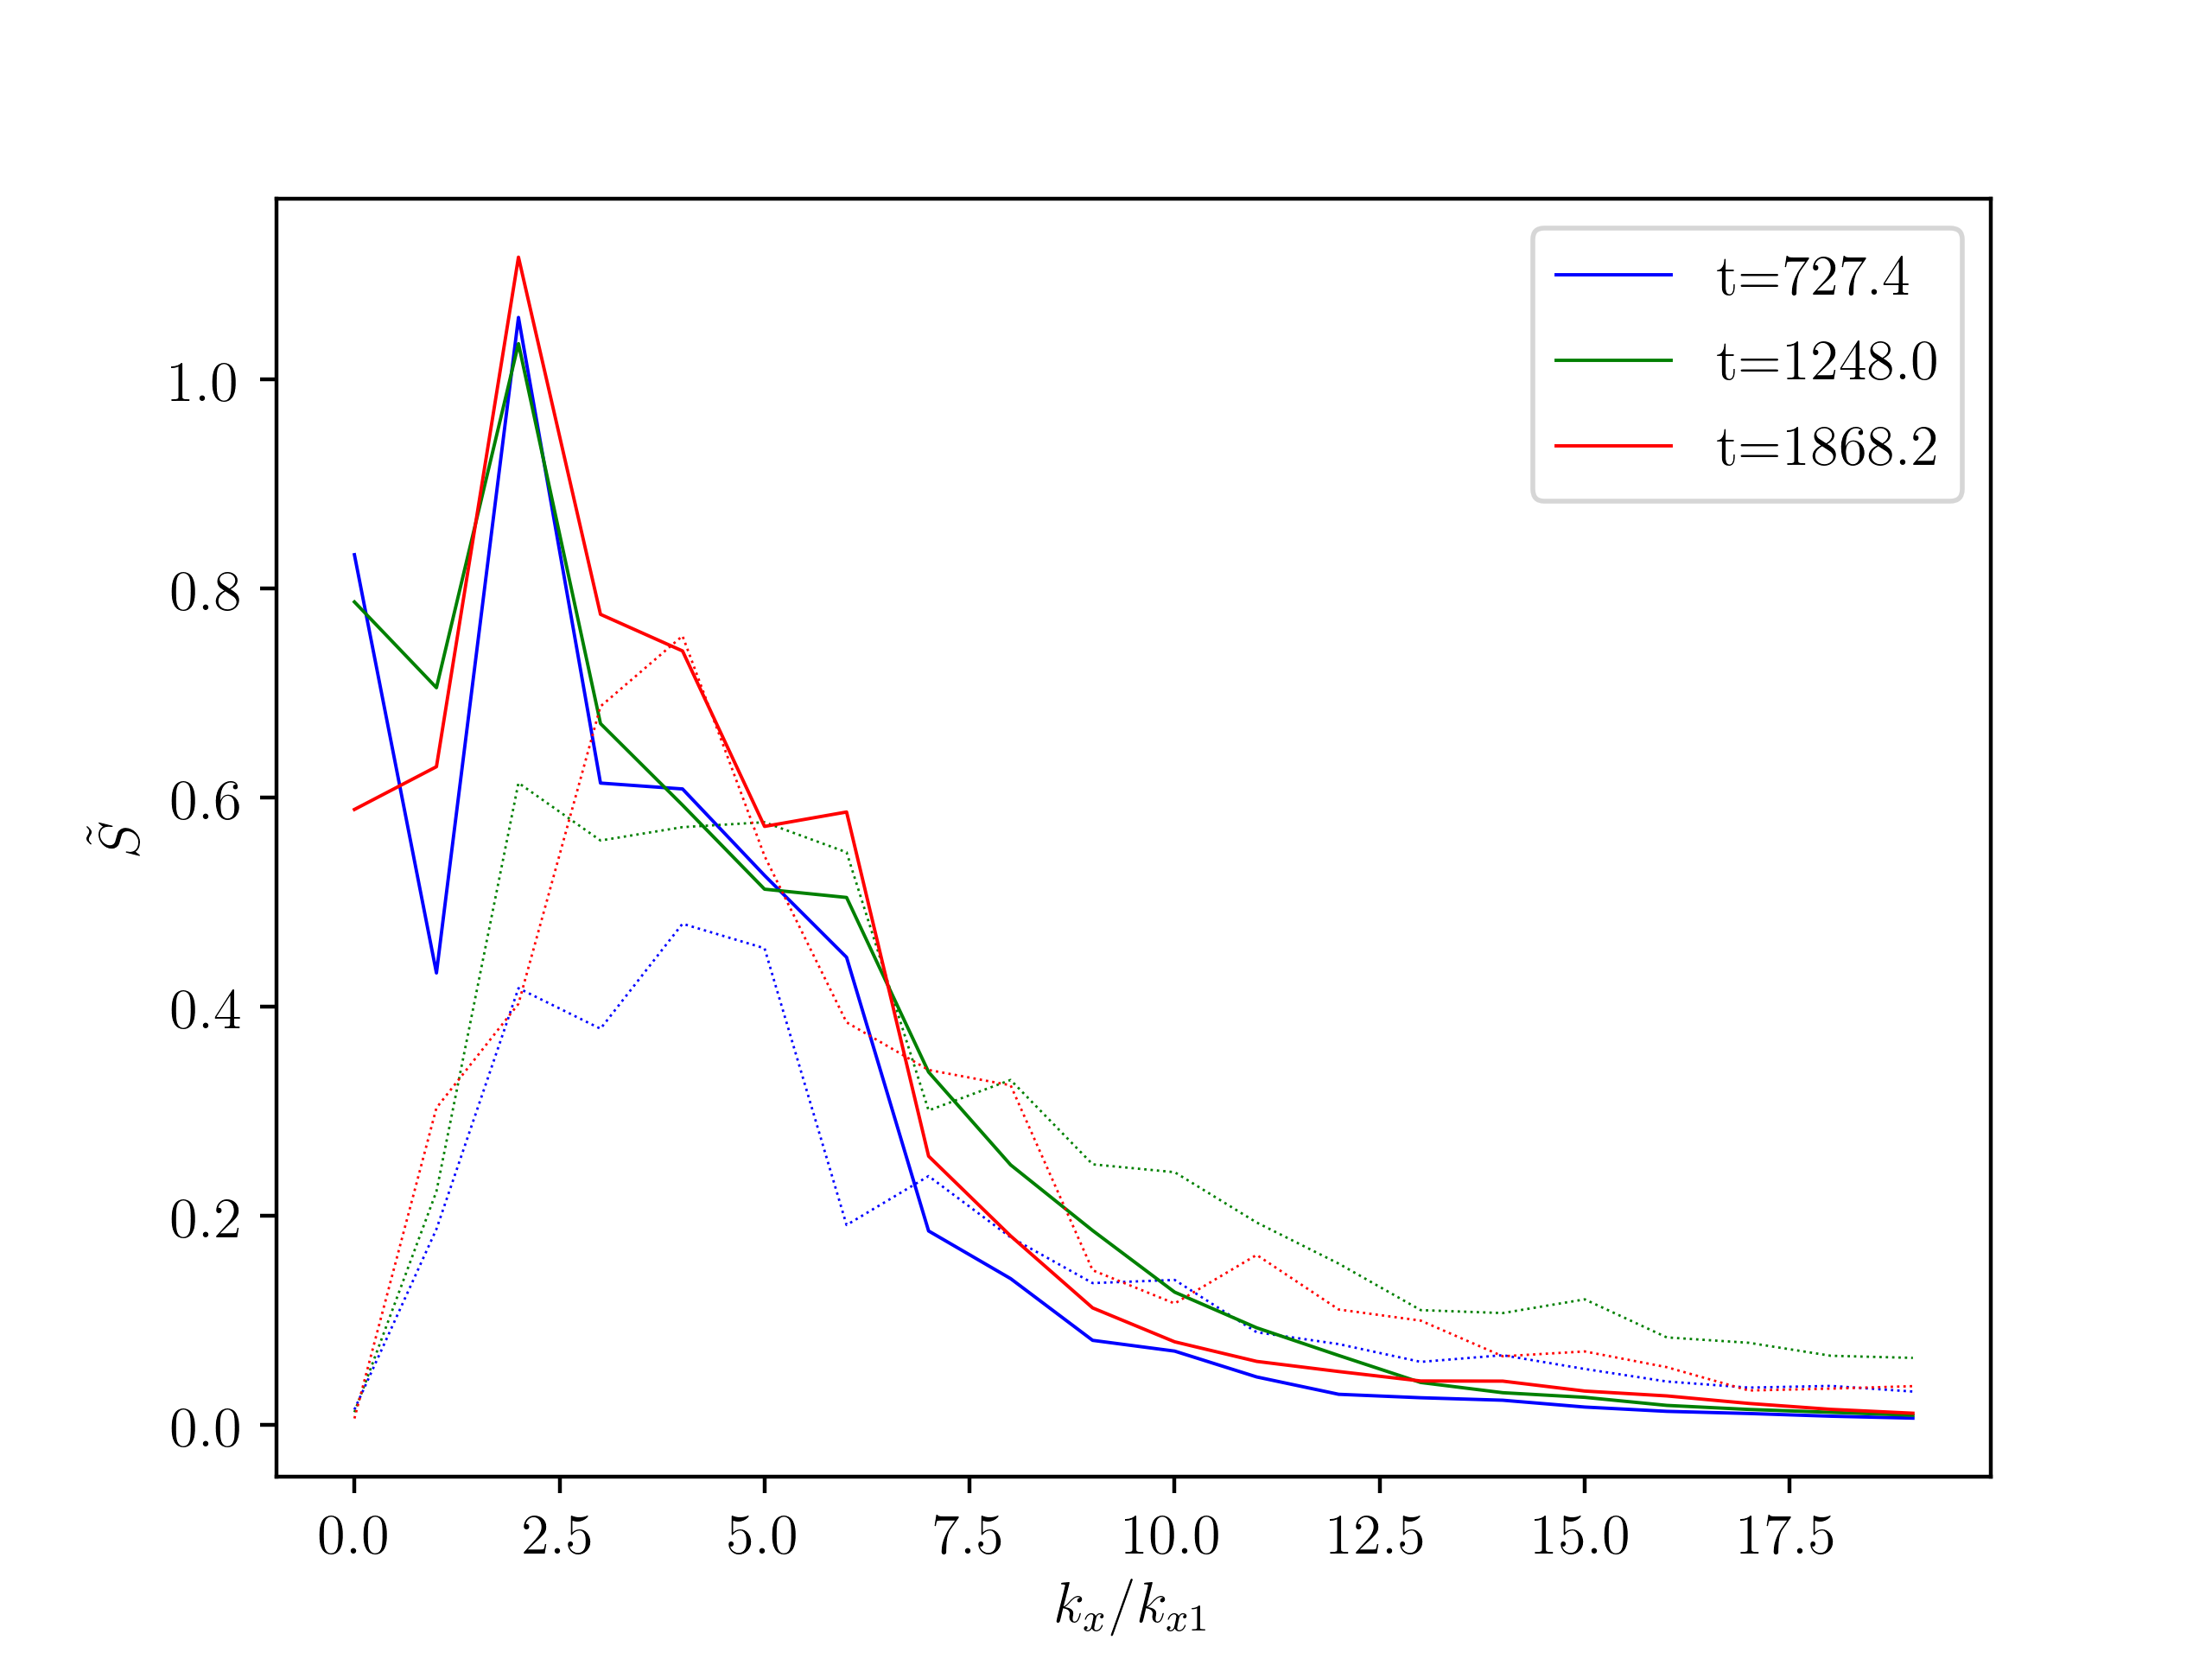
\includegraphics[width=\columnwidth]{plots/nl_fft.png}
    \caption{The power spectrum of the horizontal momentum flux at fixed
    distances below and above critical layer $z_c$ at certain times $t$ for
    simulation \texttt{0p5\_shres}. \autoref{eq:sfft_above} and
    \autoref{eq:sfft_below} are depicted here, with $\tilde{S}_<$ in solid lines
    and $\tilde{S}_>$ in dashed lines. Note that there is more incident flux
    than transmitted, and that transmitted flux roughly increases over
    time.}\label{fig:nl_fft}
\end{figure}

\subsection{Appearance of Discrete Modes}\label{ss:modes}

We briefly attribute the fluctuations in $\hat{A}_i(t)$ as observed in
\autoref{fig:nl_f_amps} to the introduction of discrete modes by partial
reflection off a moving critical layer. The partially reflecting boundary causes
a muted effect of the usual normal modes calculation, so a slightly stronger
response $\hat{A}_i > 1$ corresponds to being weakly on resonance. The
instantaneous enhancement/attenuation of $\hat{A}_i$ when $z_c$ moves slowly can
be computed by an overlap integral of the forcing with the modes of the finite
domain. This is a consistent interpretation for three reasons:
\begin{itemize}
    \item The period of the fluctuations in $\hat{A}_i(t)$ grows longer at later
        times. This is consistent with $\pd{z_c}{t}$ growing smaller at later
        times, as the critical layer propagates deeper (see
        \autoref{eq:zc_anal}).

    \item The amplitude of the fluctuations in $\hat{A}_i(t)$ grows larger at
        later times. This corresponds to the effective domain (below the
        critical layer) growing smaller, which leads to stronger boundary
        effects.

    \item The propagation time $\delta t$, defined in \autoref{eq:dt_def}, used
        the vertical phase velocity instead of the vertical group velocity to
        obtain a non-oscillating reflectivity. This is consistent with the
        fluctuations in $\hat{A}_i(t)$ being induced by internal modes of the
        domain rather than a varying forcing strength, as the latter should
        propagate at the \emph{group velocity} instead.
\end{itemize}

\section{Discussion}\label{s:discussion}

In the previous section, we have argued for a continous train of breaking IGWs
spontaneously forming a critical layer and strong shear flow. We have
parameterized the width of the critical layer as well as horizontal momentum
transport near the critical layer. In the subsequent sections, we will discuss
the validity of these results and their application to astrophysical systems.

\subsection{Convergence}\label{ss:convergence}

As the primary test of convergence in our previous sections, we consider the
convergence of the physically significant parameters of our model. In
particular, the convergence of $\mathrm{Ri}$, shown in \autoref{fig:nl_f_ri},
and of the reflection/transmission coefficient asymptotic values, shown in
\autoref{fig:nl_f_refl}, are of greatest significance.

To estimate convergence, we compute the median value of each of $\mathrm{Ri},
\mathcal{R}_A^2, \mathcal{R}_S, \mathcal{T}_S$ over the last $1/4$ of simulation
times from each simulation, where all simulations had converged to what appeared
to be asymptotic values. Error bars are estimated with the $16$ and $84$
percentiles. We illustrate the convergence of these averages across simulations
in \autoref{fig:agg}.
\begin{figure}[t]
    \centering
    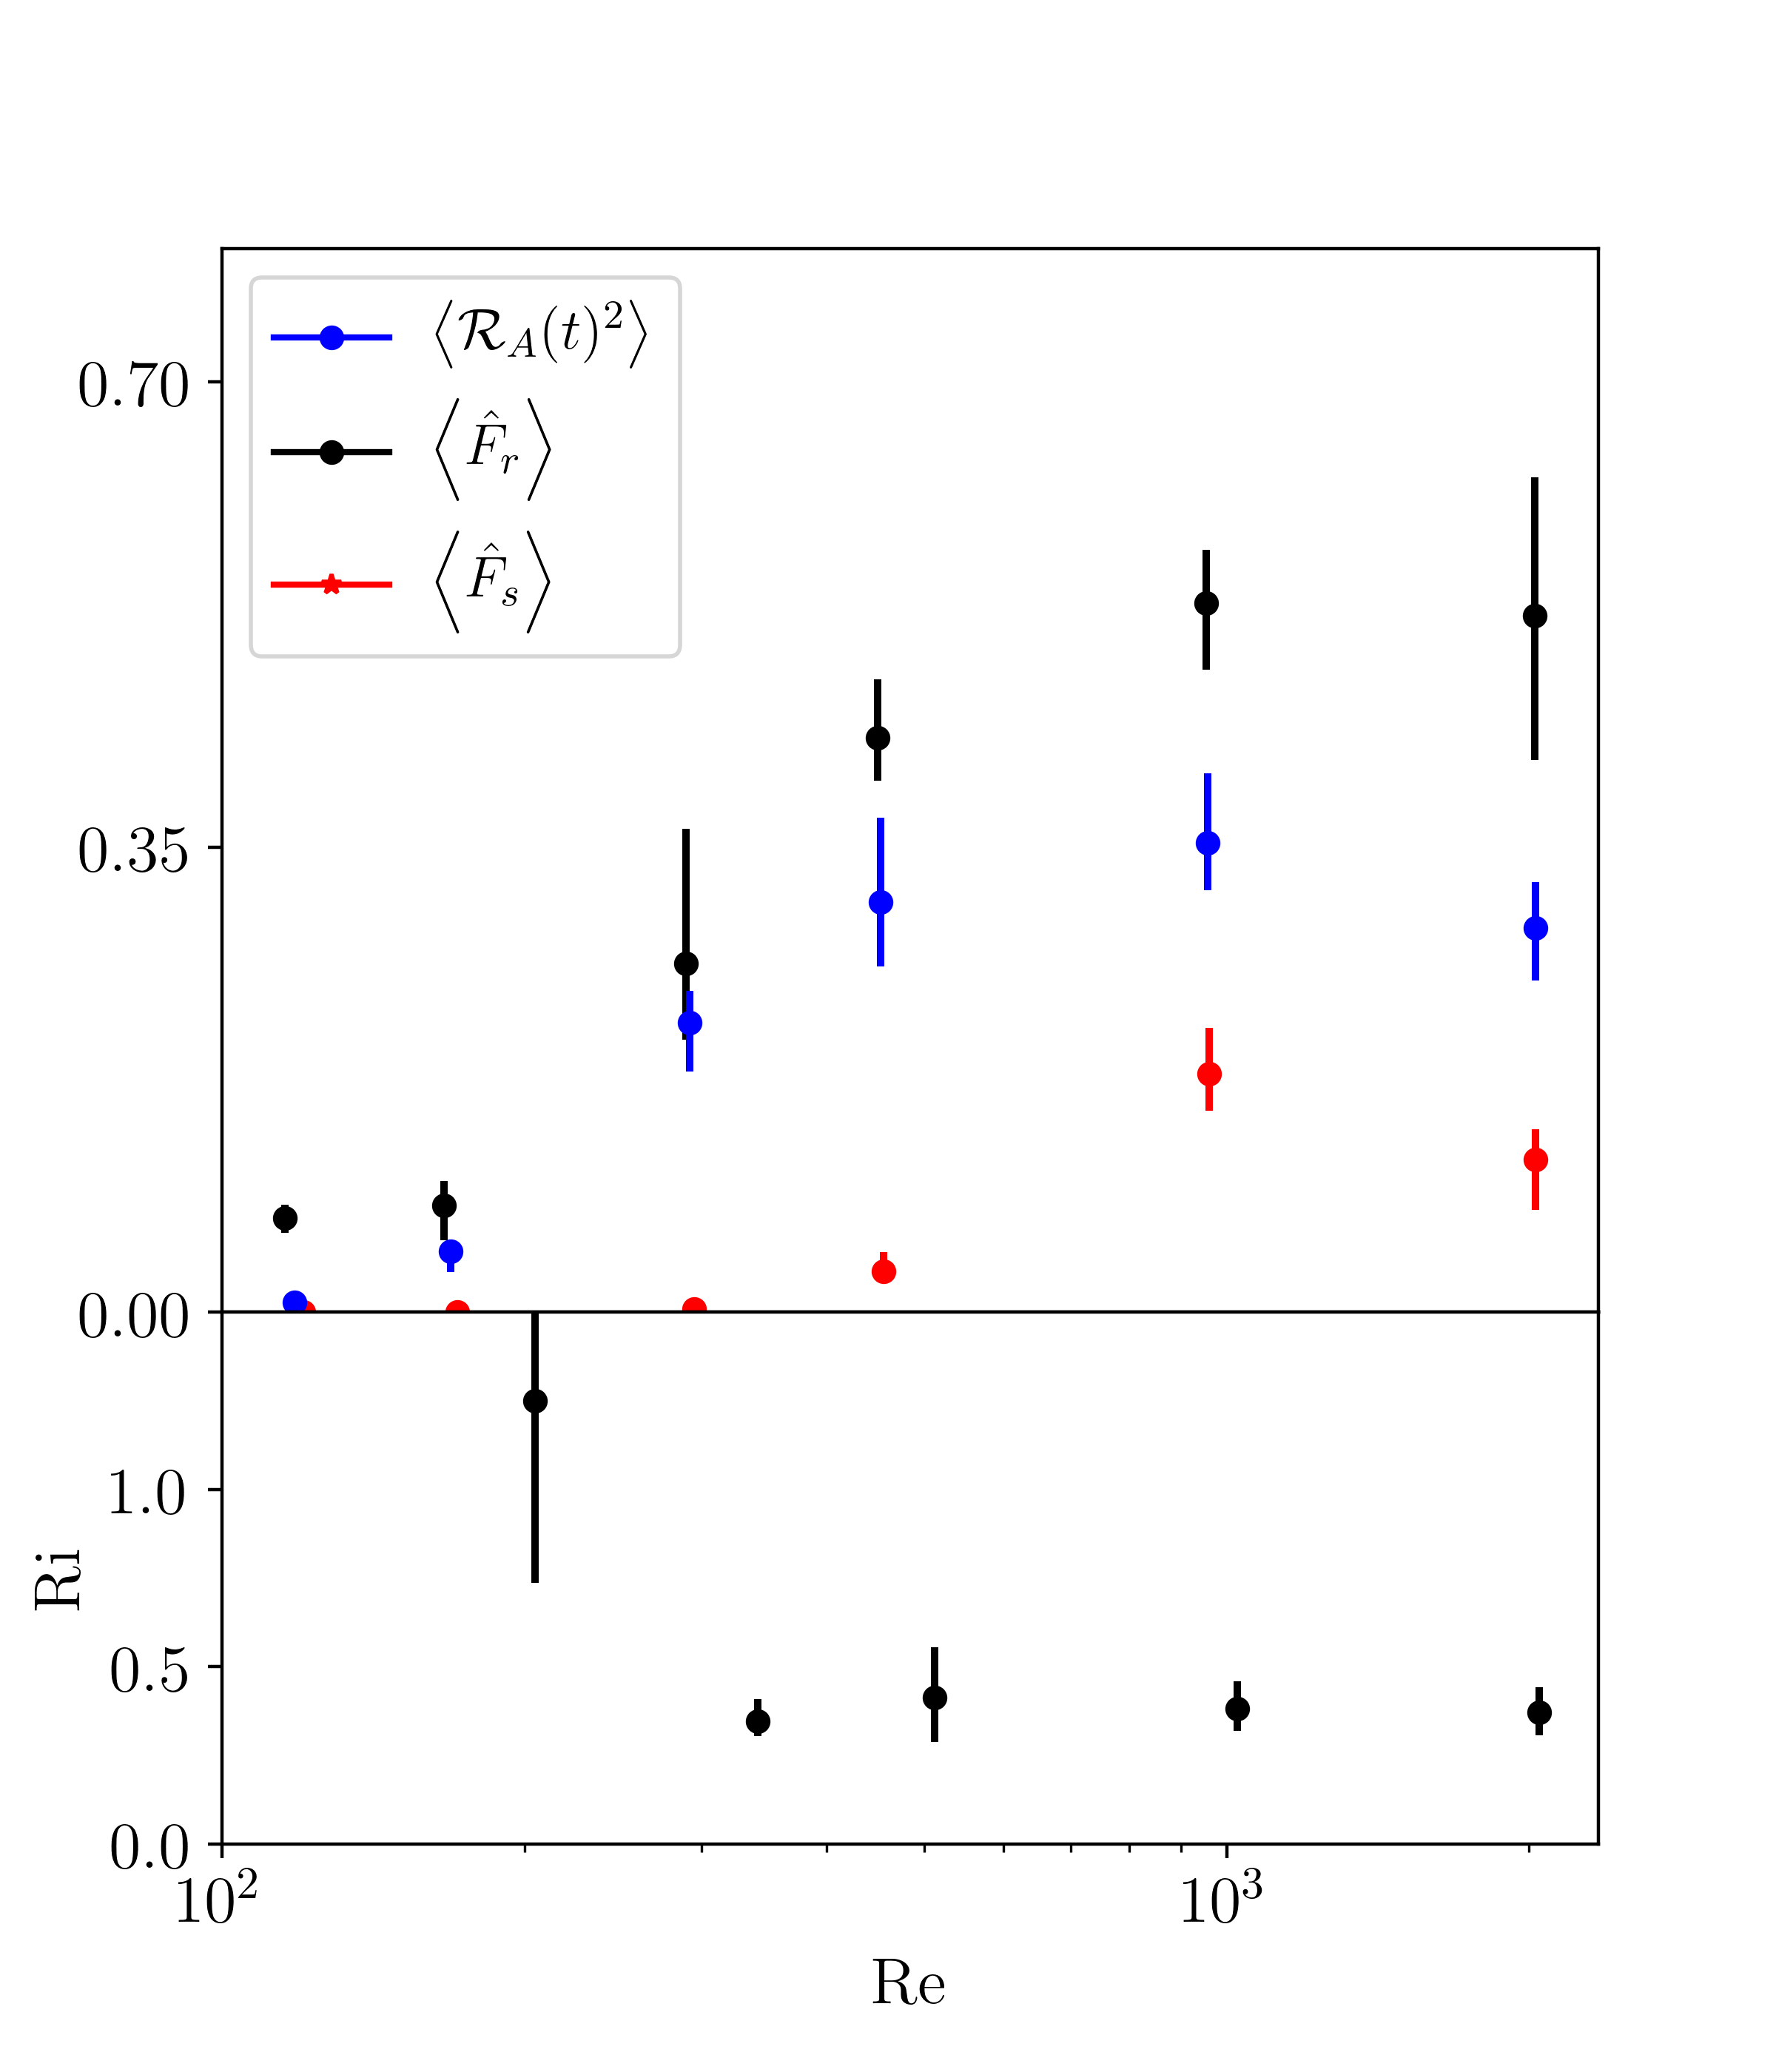
\includegraphics[width=\columnwidth]{plots/agg.png}
    \caption{Convergence of median reflection/transmission coefficients and
    $\mathrm{Ri}$ (critical layer width) across runs with varying viscosity,
    parameterized with $\mathrm{Re}$ (\autoref{eq:re_def}). Error bars depict
    $16$ and $84$ percentile values. Small horizontal displacements are made for
    data points at identical $\mathrm{Re}$ for readability. Note that
    simulations with larger $\mathrm{Re}$ correspond to smaller viscosity and
    are more physically realistic, and our values seem to converge towards large
    $\mathrm{Re}$.}\label{fig:agg}
\end{figure}

\subsection{Physical Sources of Dissipation in WDs}\label{ss:disp}

The most significant linear damping in WD g-modes comes from radiative damping
\citep{fullerI}. In \citep{wu} and \citep{fullerI}, the radiative damping rate
is given in terms of $\omega_i = \gamma \omega_r$, where $\omega_r$ is the
frequency of the g-mode. Typical values for $\gamma$ range from $10^{-4}$ to
$10^{-11}$ depending on $n$ of the g-mode.

We will assume this prescription directly transfers to propagating IGW, which
results in general agreement with \citep{bukart}'s estimate of radiative damping
rates. Then, making coarse identification $\omega_i \sim \nu k^2 \approx \nu
k_z^2$, we find that $\mathrm{Re} \sim \frac{1}{\gamma}$. Even at $\gamma =
10^{-4}$ however, the corresponding $\mathrm{Re}$ is far too weak to suppress
reflection/transmission at the critical layer (e.g.\ \autoref{fig:agg}).

Another source of dissipation considered in \citep{bukart} is turbulent
convective damping. They find this damping rate to never exceed that of
radiative damping, and so it is also too weak to suppress critical layer
formation in our problem.

Finally, we consider the impact of magnetic winding. In \citep{bukart}, magnetic
winding is used to enforce solid body rotation on the grounds that $t_A \gg
t_{gw}$, where
\begin{equation}
    t_A = \int\limits_0^R \frac{\sqrt{4\pi \rho}}{B_0}\;\mathrm{d}r
        \sim 10^2\;\mathrm{yr}\p*{\frac{10^3\;\mathrm{G}}{B}}.
\end{equation}
the Alfv\'en wave crossing time (evaluated for a CO WD in \citep{fullerIV})
measures the magnetic coupling time and $t_{gw}$ measures the gravitational wave
inspiral timescale. Before solid body rotation is attained, another relevant
timescale is the synchronization timescale $t_s$. For a tidal torque $\tau$ and
tidal forcing frequency $\sigma = m\p*{\Omega - \Omega_{spin}}$, we note that
angular momentum transfer is $\pd{M_{sync}}{t} \sigma R^2 = \tau$, where
$M_{sync}$ denotes the mass of the WD that has synchronized. Thus, the
synchronization timescale is
\begin{align}
    t_{sync} &\sim \frac{M_{sync}\sigma R^2}{\tau},\nonumber\\
        &\sim 2 \times 10^5\;\mathrm{yr}
            \p{\frac{M}{M_{\odot}}}
            \p{\frac{\sigma}{2\pi / (1\;\mathrm{hr})}}
            \p{\frac{R}{R_{\oplus}}}^2
            \p{\frac{10^{-14} GM_{\odot}^2/R_{\oplus}}{\tau}}.
\end{align}
A representative $\tau$ has been taken from \citep{bukart}. However, since only
the outer $\sim 10^{-4}M_{\odot}$ need be heated for the thermodynamically
interesting effects studied in \citep{fullerIV} and \citep{tidal_novae}, it
seems that magnetic winding cannot absolutely rule out energetic outbursts such
as tidal novae resulting from strong shear flows.

\subsection{Applicability to Other Astrophysical Systems}

[TODO flesh out]

\begin{itemize}
    \item $k_x, k_z$: In astrophysical systems, $k_{\perp} \ll k_r$. While we do
        not explore different $k_{1x}, k_{1z}, \omega_1$ in this study, with
        outgoing boundary conditions, there appears at first to be no $z$ length
        scale other than $k_{1z}$, so our results would seem to be invariant
        under rescaling of the $z$ length scale. However, true turbulence is
        expected to be isotropic at small scales, which may couple $k_{1x},
        k_{1z}$ in a way that $k_{1x} \ll k_{1z}$ produces different dynamics
        than $k_{1x} \lesssim k_{1z}$ as we've studied. This is a numerically
        difficult regime though, so we defer consideration to future work.

    \item Validity of plane-parallel approximation? We're all at $\gtrsim
        0.9R_{WD}$.

    \item Solar-type stars (inner convective, outer radiative): different
        equation of state/stratification but could be qualitatively similar.

    \item Solar-type stars: In~\cite{barker_ogilvie}, inwards-propagating IGW
        are excited that break via geometric focusing and effect
        synchronization. They find no reflected wave despite their nonlinear
        timescales being $10\times$ shorter than their viscous timescale.

        It is not immediately clear whether our results here apply when the flux
        is geometrically focused, but as a hypothesis we assume the convergence
        in \autoref{fig:agg} applies under geometric focusing as a zeroth
        approximation, perhaps as a property of the fluid motion within the
        geometrically thin critical layer.

        Associating $t_{} \sim \nu k^2 \approx \nu k_z^2$ with the visocus
        timescale and $t_{NL} \sim \vec{u} \cdot \vec{\nabla} \sim \omega$ for
        the nonlinear timescale, we find their $\lambda = \frac{t_{NL}}{t_L}
        \sim \mathrm{Re}$ our Reynolds number. Our simulations indicate
        $\mathrm{Re} \gtrsim 500$ are required to observe the correct asymptotic
        behavior in terms of horizontal momentum flux reflection/transmission,
        so it is possible their lack of reflection is viscosity limited.
\end{itemize}

\subsection{Heating}

[TODO elaborate? Need to make plots to check?]

Our equations do not conserve energy, but it seems like more energy can be
transmitted in higher modes as viscosity is decreased. Nevertheless, a
significant fraction should still be dissipated in the critical layer since a
significant energy cascade must happen in the critical layer.

\section{Acknowledgements}\label{s:ack}

\bibliographystyle{mnras}
\bibliography{paper}

\clearpage
\onecolumn
\appendix

\section{Equation Implementations}\label{ss:strat_impl}

We denote $x \in [0, L_x], z \in [0, L_z]$ the simulation domain and $N_x, N_z$
the number of spectral modes in the respective dimensions.

Numerically, the nonlinear $\frac{\vec{\nabla}P}{\rho}$ term is problematic: we
desire a system where the fluid fields are not divided by one another. We
introduce $\varpi = \frac{P}{\rho}$ instead, then mandate $\rho_0, \varpi_0$
background fields satisfy hydrostatic equilibrium $\vec{\nabla}\varpi_0 +
\varpi_0 \vec{\nabla}\rho_0 + g\hat{z} = 0$. Taking isothermal stratification,
we find $\varpi_0 = gH$. We further change variables to $\Upsilon = \ln \rho -
\ln \rho_0$ and $\varpi_1 = \varpi - \varpi_0$ deviations from the background
state to obtain a system of equations at most quadratic in fluid fields:
\begin{subequations}\label{se:nl_var}
    \begin{align}
        \vec{\nabla} \cdot \vec{u}_1 &= 0,\\
        \pd{\Upsilon}{t} + \p{\vec{u}_1 \cdot \vec{\nabla}} \Upsilon
            - \frac{u_z}{H} &= 0,\\
        \pd{u_{1x}}{t} + \p{\vec{u}_1 \cdot \vec{\nabla}}u_{1x}
            + \pd{\varpi_1}{x} + gH\pd{\Upsilon}{x}
            + \varpi_1 \pd{\Upsilon}{x} &= 0,\\
        \pd{u_z}{t} + \p{\vec{u}_1 \cdot \vec{\nabla}}u_z
            + \pd{\varpi_1}{z} + gH\pd{\Upsilon}{z}
            + \varpi_1 \pd{\Upsilon}{z} - \frac{\varpi_1}{H} &= 0.
    \end{align}
\end{subequations}
It bears noting that these equations are exactly equivalent to the original
Euler equations and hence conserve horizontal momentum.

\subsection{Artificial Dissipation}

The nonlinear terms in the above equations will transfer energy from lower
wavenumbers to higher wavenumbers. Since spectral codes have no numerical
dissipation, artificial dissipation must be added. To ensure the dissipitive
system conserves horizontal momentum, we begin by adding dissipitive terms to
the flux-conservative form of the Euler fluid equations \autoref{se:nl_orig} (we
use stress tensor $\tau_{ij} = P\delta_{ij}$):
\begin{subequations}
    \begin{align}
        \vec{\nabla} \cdot \vec{u} &= 0,\\
        \partial_t \rho + \vec{\nabla} \cdot (\rho \vec{u} - \nu
            \vec{\nabla}(\rho - \rho_0)) &= 0,\label{eq:visc_cons_mom}\\
        \partial_t (\rho \vec{u}) + \vec{\nabla} \cdot (\rho \vec{u}
        \vec{u} +
            \mathrm{diag}(\rho \varpi) - \nu \rho \vec{\nabla}\vec{u}) + \rho g
            \hat{z} &= 0.
    \end{align}
\end{subequations}
The same $\nu$ is used for both the diffusive and viscous term, though this is
not required. Since the dissipation is not physical and is purely used for
numerical stability, we choose it such that hydrostatic equilibrium is not
modified. Some algebraic manipulation to re-cast it in the form of
\autoref{se:nl_var} gives
\begin{subequations}
    \begin{align}
        \vec{\nabla} \cdot \vec{u} &= 0,\\
        \partial_t \Upsilon + \p{\vec{u} \cdot \vec{\nabla}} \Upsilon -
            \frac{u_z}{H} - \nu\p{\nabla^2 \Upsilon + \p{\vec{\nabla}
            \Upsilon} \cdot \p{\vec{\nabla}\Upsilon} - \frac{2}{H}\partial_z
            \Upsilon + \frac{1 - e^{-\Upsilon}}{H^2}} &= 0,\\
        \partial_t \vec{u} + \p{\vec{u} \cdot \vec{\nabla}}\vec{u} +
            \vec{\nabla} \varpi + \varpi \vec{\nabla} \Upsilon - \nu \nabla^2
            \vec{u} + \vec{u} \nu\p{\nabla^2 \Upsilon + \p{\vec{\nabla}
            \Upsilon} \cdot \p{\vec{\nabla}\Upsilon} - \frac{2}{H}\partial_z
            \Upsilon + \frac{1 - e^{-\Upsilon}}{H^2}}&{}\nonumber\\
        - 2\nu \p{\p{\p{\vec{\nabla}\Upsilon} \cdot \vec{\nabla}}\vec{u} -
            \frac{1}{H}\partial_z \vec{u}} - \frac{\varpi_1}{H} &= 0.
    \end{align}
\end{subequations}
Hydrostatic equilibrium is still $\vec{\nabla} \varpi_0 + g\hat{z} = 0$ where
$\rho = \rho_0, \vec{u} = 0$. Including the damping layers and forcing terms as
described in \autoref{ss:numerics}, we finally obtain the full system of
equations as simulated in Dedalus:
\begin{subequations}
    \begin{align}
        \vec{\nabla} \cdot \vec{u} ={}& 0,\\
        \partial_t \Upsilon - \frac{u_z}{H}
            ={}& \nu\p{\nabla^2 \Upsilon + \p{\vec{\nabla}
            \Upsilon} \cdot \p{\vec{\nabla}\Upsilon} - \frac{2}{H}\partial_z
            \Upsilon + \frac{1 - e^{-\Upsilon}}{H^2}},\nonumber\\
            & - \p{\vec{u} \cdot \vec{\nabla}}\Upsilon
                -\Gamma(z) \Upsilon
                + \frac{F}{\rho_0(z)}e^{-\frac{(z - z_0)^2}{2\sigma^2}}
                    \cos \p{k_xx - \omega t},\\
        \pd{u_x}{t} + \pd{T}{x} + gH\pd{\Upsilon}{x} ={}&
            \nu \nabla^2 u_x
            - u_x \nu\p{\nabla^2 \Upsilon + \p{\vec{\nabla} \Upsilon} \cdot
                \p{\vec{\nabla}\Upsilon} - \frac{2}{H}\partial_z \Upsilon
                + \frac{1 - e^{-\Upsilon}}{H^2}}\nonumber\\
            &+ 2\nu \p{\p{\p{\vec{\nabla}\Upsilon} \cdot \vec{\nabla}}u_x
                - \frac{1}{H}\partial_z u_x}
            -\Gamma(z) u_x
                - \p{\vec{u} \cdot \vec{\nabla}}u_x
                - T_1 \pd{\Upsilon}{x},\\
        \pd{u_z}{t} + \pd{T}{z} + gH\pd{\Upsilon}{z} - \frac{T_1}{H} ={}&
            \nu \nabla^2 u_z
            - u_z \nu\p{\nabla^2 \Upsilon + \p{\vec{\nabla} \Upsilon} \cdot
                \p{\vec{\nabla}\Upsilon} - \frac{2}{H}\partial_z \Upsilon
                + \frac{1 - e^{-\Upsilon}}{H^2}}\nonumber\\
            &+ 2\nu \p{\p{\p{\vec{\nabla}\Upsilon} \cdot \vec{\nabla}}u_z -
                \frac{1}{H}\partial_z u_{z}}
            -\Gamma(z) u_z - \p{\vec{u} \cdot \vec{\nabla}}u_z
            - T_1 \pd{\Upsilon}{z}.
    \end{align}
\end{subequations}
\label{lastpage} % chktex 24
\end{document}
